%\renewcommand\thefigure{\thesection.\arabic{figure}}   
%\renewcommand\thetable{\thesection.\arabic{figure}}
\counterwithin{figure}{section}
\counterwithin{table}{section}

\begin{appendices}
	%	\addtocontents{lof}{\protect\contentsline{chapter}{%
			%			Appendices \vspace{10pt}
			%	}{}
%		\addtocontents{toc}{\protect\setcounter{tocdepth}{1}}
%		\makeatletter
%		\addtocontents{toc}{%
%			\begingroup
%			\let\protect\l@chapter\protect\l@section
%			\let\protect\l@section\protect\l@subsection
%		}
%		\makeatother
		
%		\huge{\textbf{All File Operations Firefox}}
%%		\enlargethispage{6cm}

%		
%		\huge{\textbf{All File Operations Tor}}
%%		\enlargethispage{6cm}
%		\begin{figure}[h!]
%			\centerline{\resizebox{!}{0.9\textheight}{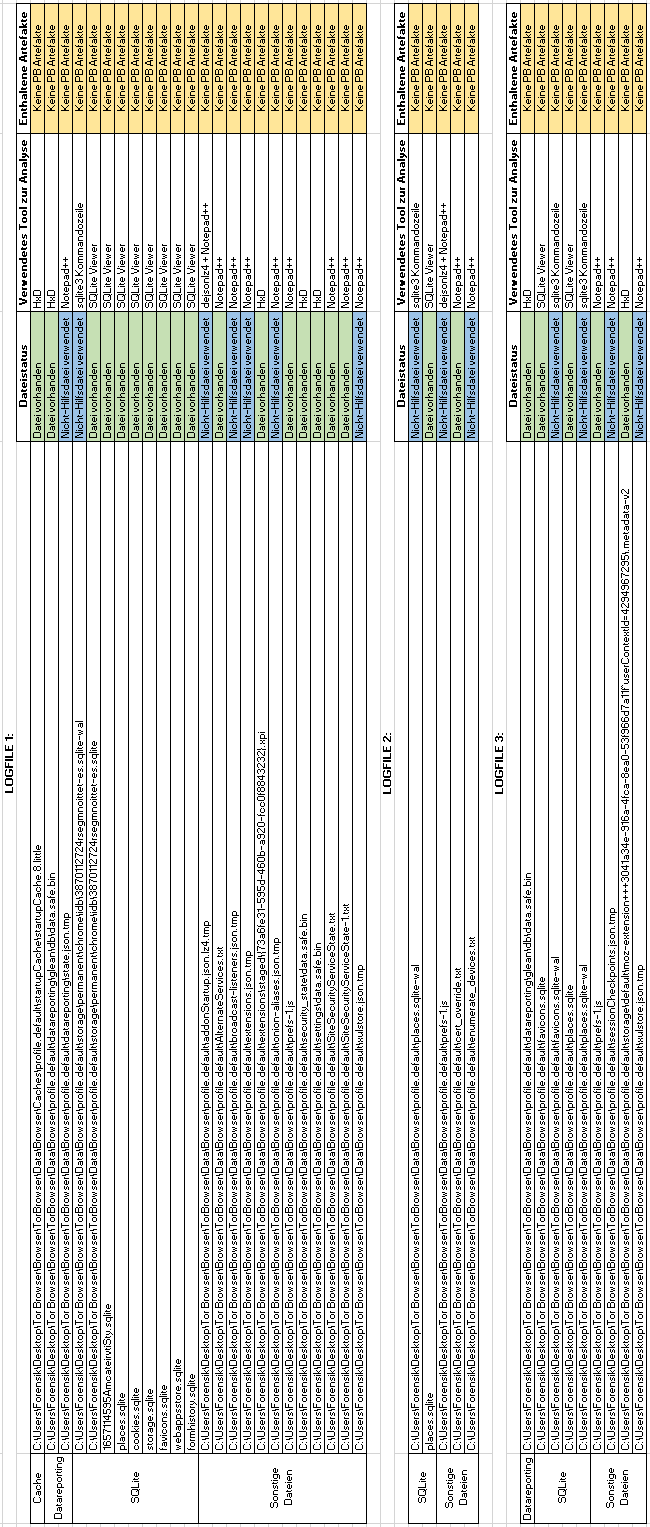
\includegraphics{bilder/tor-all-write-operations.png}}}
%			%	\label{...}
%			\caption{All File Operations Firefox: Logfile 1 vs. Logfile 2 vs. Logfile 3}
%		\end{figure}

\renewcommand{\thesection}{\Alph{section}}

\newgeometry{left=1.5cm,bottom=2cm,top=0.5cm}
\begin{landscape}% Landscape page
	\section{Yara-Regeln}
	\label{appendix:yara-regeln}
	\setcounter{page}{43}
%	\thispagestyle{empty}
	\vspace*{-0.5cm}
%	\hspace*{-1cm}
\begin{multicols}{2}
		\begin{minted}[
			obeytabs=true,
			tabsize=2,
			autogobble,
			fontsize=\footnotesize,
			frame=single
			]{text}
			rule keyword {
				strings:
					$pfaffenhofen_keyword="pfaffenhofen" wide ascii nocase
					$nanoradar_keyword="nanoradar" wide ascii nocase	
				condition:
					$pfaffenhofen_keyword or $nanoradar_keyword 
			}
			
			rule keyword_mooserliesl {
				strings:
					$mooserliesl1_keyword="mooserliesl" wide ascii nocase
					$mooserliesl1_keyword2="mooserliesl.de" wide ascii nocase	
				condition:
					$mooserliesl1_keyword and not $mooserliesl1_keyword2
			}
			
			rule keyword_mallofamerica {
				strings:		
					$mallofamerica1_keyword="mallofamerica" wide ascii nocase
					$mallofamerica1_keyword2="mallofamerica.com" wide ascii nocase	
				condition:
					$mallofamerica1_keyword and not $mallofamerica1_keyword2
			}
			
			rule url {
				strings:
					$mallofamerica_url="mallofamerica.com" wide ascii nocase
					$mooserliesl_url="mooserliesl.de" wide ascii nocase
					$unitree_url="unitree.com" wide ascii nocase
					$donaukurier_url="donaukurier.de" wide ascii nocase	
				condition:
					$mallofamerica_url or $mooserliesl_url or $unitree_url or $donaukurier_url
			}
			
			rule html {
				strings:			
					$mallofamerica_html="Insiders</span>" wide ascii nocase
					$mooserliesl_html="Ja</span>" wide ascii nocase
					$unitree_html="L1</div>" wide ascii nocase
					$donaukurier_html=">Themen:" wide ascii nocase		
				condition:
					$mallofamerica_html or $mooserliesl_html or $unitree_html or $donaukurier_html
			}
			
			rule image {
				strings:
					$image_hex = {89 50 4E 47 0D 0A 1A 0A 00 00 00 0D 49 48 44 52 00 00 01 2C 00 00 
								  00 32 08 03 00 00 00 D1 08 16 18 00 00 00 19 74 45 58 74 53 6F 66 
								  74 77 61 72 65 00 41 64 6F 62 65 20 49 6D 61 67 65 52 65 61 64 79 
								  71 C9 65 3C 00 00 03 84 69 54 58 74 58 4D 4C 3A 63 6F 6D 2E 61 64 
								  6F 62 65 2E 78 6D 70 00 00 00 00 00 3C 3F 78 70 61 63 6B 65 74 20 
																 ...
								  4E AD 38 61 03 55 6A AB 5E BF F6 40 4E 9D BA 20 FE 43 FE 99 81 2C 
								  0A 8F B2 F1 D8 7B DE E5 75 7E 45 E3 FC E4 C8 81 E5 C0 72 60 39 B0 
								  1C 71 60 39 B0 1C 58 0E 2C 07 D6 FF A9 FC 57 80 01 00 D9 B2 CD 5E 
								  42 B8 37 25 00 00 00 00 49 45 4E 44 AE 42 60 82}
				condition:
					$image_hex
			}
			
			rule mail {
				strings:		
					$computerforensik_address="computerforensikvl@gmail.com" wide ascii nocase
					$computerforensik_password="Vorlesung23!" wide ascii nocase
					$cas0597_address="cas0597@thi.de" wide ascii nocase
					$chs3702_address="chs3702@thi.de" wide ascii nocase
					$subject="Betrefftext" wide ascii nocase
					$mail_body="Mailinhalt" wide ascii nocase	
				condition:
					$computerforensik_address or $computerforensik_password or $cas0597_address or 
					$chs3702_address or $subject or $mail_body
			}
		\end{minted}
\end{multicols}
%%	\vspace{-1cm}
%	\caption{Yara-Regeln}
%	\label{code:yara-rule}
\end{landscape}
\restoregeometry

\section{Ausführliche Analyse: Firefox}
\subsection{Common Locations}
\label{subsection:appendix-firefox-common-locations}
\subsubsection*{Process Monitor WriteFile Operations}
\label{subsubsection:appendix-firefox-common-locations-writefile-operations}
Gemäß Versuchsdurchführung wurden für Firefox mit dem Process Monitor Tool zwei Logfiles erstellt. Diese Dateien enthalten alle aufgezeichneten Prozessaktivitäten während und nach dem Browsing Szenario.
Zunächst wurden die beiden Logfiles gemäß Methodik in Kapitel \ref{subsection:methodik-datensammlung-processmonitorlogfiles} in Excel aufbereitet. Tabelle \ref{tab:firefox-writefile-operations} listet alle in den gefilterten Logfiles identifizierten Dateien auf. Dabei wurde für jede Datei vermerkt, ob und wie sie wiederherstellbar war, mit welchem Tool die Datei analysiert wurde und ob in der Datei PB Artefakte enthalten sind. Die wiederherstellbaren Dateien wurden in die fünf Kategorien \textit{Cache}, \textit{Datareporting}, \textit{Sessionstore-Backup} und \textit{Sonstige Dateien} eingeordnet. In keiner der Dateien wurden PB Artefakte identifiziert.

Bei detaillierter Untersuchung der wiederherstellbaren Dateien konnten zwei Pfade identifiziert werden, in die Firefox während des Versuchs Dateien schreibt. 
\begin{itemize}
\item[\textbf{Local}] \texttt{C:$\backslash$Users$\backslash$<User>$\backslash$AppData$\backslash$Local$\backslash$Mozilla$\backslash$Firefox$\backslash$Profiles$\backslash$<Profile>.default-release$\backslash$}
\item[\textbf{Roaming}] \texttt{C:$\backslash$Users$\backslash$<User>$\backslash$AppData$\backslash$Roaming$\backslash$Mozilla$\backslash$Firefox$\backslash$Profiles$\backslash$<Profile>.default-release$\backslash$}
\end{itemize}
In Tabelle X (TODO!) sind die Dateien je nach Speicherort \textit{Local} (Hellblau) oder \textit{Roaming} (Dunkelblau) entsprechend eingefärbt. Ausschließlich Dateien der Kategorie ``Cache`` sind im Local Pfad gespeichert.

\paragraph*{Cache}
Firefox verwendet den Cache, um Webseiten und deren Ressourcen temporär lokal zu speichern. Dadurch können wiederholte Anfragen an den Server vermieden und die Ladezeiten verringert werden. Die Inhalte dieser Dateien sind binär.
Die Cache-Dateien im Format \texttt{$\backslash$cache2$\backslash$entries$\backslash$<ID>} werden im Local Pfad gespeichert.

%\newpage
\newgeometry{bottom=2cm,top=0.5cm}
%\setcounter{figure}{0}    
\afterpage{
\begin{landscape}% Landscape page
	\setcounter{page}{43}
%	\thispagestyle{empty}
	\vspace*{1.5cm}
	\hspace*{-1cm}
	\begin{table}[h!]
%	\centering
	\caption{Firefox alle ``WriteFile``-Operationen der Logfiles 1 und 2}
	\label{tab:firefox-writefile-operations}
	\vspace{0.5cm}
	\resizebox{\linewidth}{!}{
	\begin{tabular}{cllll}
	\multicolumn{5}{c}{\textbf{LOGFILE 1:}}                                                                                                                                                                                                                                                                                                                                                                                                                                                                                                                     \\ \hline
	\multicolumn{1}{|c|}{\textbf{Kategorie}}                                                                     & \multicolumn{1}{c|}{\textbf{Dateiname}}                                                                                                                                                                             & \multicolumn{1}{c|}{\textbf{Dateistatus}}                                                         & \multicolumn{1}{c|}{\textbf{Tool für Analyse}}   & \multicolumn{1}{l|}{\textbf{Enthaltene Artefakte}}              \\ \hline
	\multicolumn{1}{|c|}{}                                                                                       & \multicolumn{1}{l|}{\cellcolor[HTML]{34CDF9}\textbackslash{}cache2\textbackslash{}entries\textbackslash{}037778A55E1B7E9BED3390289866D09402D6C913}                                                                  & \multicolumn{1}{l|}{\cellcolor[HTML]{009901}Datei vorhanden}                                      & \multicolumn{1}{l|}{MozillaCacheView}            & \multicolumn{1}{l|}{\cellcolor[HTML]{F8A102}Keine PB Artefakte} \\ \cline{2-5} 
	\multicolumn{1}{|c|}{}                                                                                       & \multicolumn{1}{l|}{\cellcolor[HTML]{34CDF9}\textbackslash{}cache2\textbackslash{}entries\textbackslash{}1223A0378B8971FA4CD25EA1731C80B2B1676B42}                                                                  & \multicolumn{1}{l|}{\cellcolor[HTML]{009901}Datei vorhanden}                                      & \multicolumn{1}{l|}{MozillaCacheView}            & \multicolumn{1}{l|}{\cellcolor[HTML]{F8A102}Keine PB Artefakte} \\ \cline{2-5} 
	\multicolumn{1}{|c|}{}                                                                                       & \multicolumn{1}{l|}{\cellcolor[HTML]{34CDF9}\textbackslash{}cache2\textbackslash{}entries\textbackslash{}250EE2BC03AFF526F1A1C3DB212A79DE3EB60D5E}                                                                  & \multicolumn{1}{l|}{\cellcolor[HTML]{009901}Datei vorhanden}                                      & \multicolumn{1}{l|}{MozillaCacheView}            & \multicolumn{1}{l|}{\cellcolor[HTML]{F8A102}Keine PB Artefakte} \\ \cline{2-5} 
	\multicolumn{1}{|c|}{}                                                                                       & \multicolumn{1}{l|}{\cellcolor[HTML]{34CDF9}\textbackslash{}jumpListCache\textbackslash{}ZKJGVJPzPe7w4w0KwEY0jw==.ico}                                                                                              & \multicolumn{1}{l|}{\cellcolor[HTML]{009901}Datei vorhanden}                                      & \multicolumn{1}{l|}{Windows Foto App}            & \multicolumn{1}{l|}{\cellcolor[HTML]{F8A102}Keine PB Artefakte} \\ \cline{2-5} 
	\multicolumn{1}{|c|}{}                                                                                       & \multicolumn{1}{l|}{\cellcolor[HTML]{34CDF9}\textbackslash{}cache2\textbackslash{}entries\textbackslash{}D16E4E5DFB15B4C8DE88842C05A47A07C611E01D}                                                                  & \multicolumn{1}{l|}{\cellcolor[HTML]{009901}Datei vorhanden}                                      & \multicolumn{1}{l|}{MozillaCacheView}            & \multicolumn{1}{l|}{\cellcolor[HTML]{F8A102}Keine PB Artefakte} \\ \cline{2-5} 
	\multicolumn{1}{|c|}{\multirow{-6}{*}{\textit{Cache}}}                                                       & \multicolumn{1}{l|}{\cellcolor[HTML]{34CDF9}\textbackslash{}cache2\textbackslash{}entries\textbackslash{}2F040683A85A4372A73572713C6C52B510854566}                                                                  & \multicolumn{1}{l|}{\cellcolor[HTML]{009901}Datei vorhanden}                                      & \multicolumn{1}{l|}{MozillaCacheView}            & \multicolumn{1}{l|}{\cellcolor[HTML]{F8A102}Keine PB Artefakte} \\ \hline
	\multicolumn{1}{|c|}{}                                                                                       & \multicolumn{1}{l|}{\cellcolor[HTML]{3190FF}\textbackslash{}datareporting\textbackslash{}glean\textbackslash{}events\textbackslash{}pageload}                                                                       & \multicolumn{1}{l|}{\cellcolor[HTML]{009901}Datei vorhanden}                                      & \multicolumn{1}{l|}{HxD}                         & \multicolumn{1}{l|}{\cellcolor[HTML]{F8A102}Keine PB Artefakte} \\ \cline{2-5} 
	\multicolumn{1}{|c|}{}                                                                                       & \multicolumn{1}{l|}{\cellcolor[HTML]{3190FF}\textbackslash{}datareporting\textbackslash{}glean\textbackslash{}db\textbackslash{}data.safe.tmp}                                                                      & \multicolumn{1}{l|}{\cellcolor[HTML]{FCFF2F}Nicht-temp-Datei verwendet}                           & \multicolumn{1}{l|}{HxD}                         & \multicolumn{1}{l|}{\cellcolor[HTML]{F8A102}Keine PB Artefakte} \\ \cline{2-5} 
	\multicolumn{1}{|c|}{}                                                                                       & \multicolumn{1}{l|}{\cellcolor[HTML]{3190FF}\textbackslash{}datareporting\textbackslash{}glean\textbackslash{}tmp\textbackslash{}95ea3e10-e732-4642-8e92-515f4c4e090c}                                              & \multicolumn{1}{l|}{\cellcolor[HTML]{963400}{\color[HTML]{FFFFFF} Datei nicht wiederherstellbar}} & \multicolumn{1}{l|}{\cellcolor[HTML]{C0C0C0}N/A} & \multicolumn{1}{l|}{\cellcolor[HTML]{C0C0C0}N/A}                \\ \cline{2-5} 
	\multicolumn{1}{|c|}{\multirow{-4}{*}{\textit{Datareporting}}}                                               & \multicolumn{1}{l|}{\cellcolor[HTML]{3190FF}\textbackslash{}datareporting\textbackslash{}glean\textbackslash{}tmp\textbackslash{}16ab2ae2-c7b8-4390-a26e-7dcd95f5ff24}                                              & \multicolumn{1}{l|}{\cellcolor[HTML]{963400}{\color[HTML]{FFFFFF} Datei nicht wiederherstellbar}} & \multicolumn{1}{l|}{\cellcolor[HTML]{C0C0C0}N/A} & \multicolumn{1}{l|}{\cellcolor[HTML]{C0C0C0}N/A}                \\ \hline
	\multicolumn{1}{|c|}{\textit{Sessionstore}}                                                                  & \multicolumn{1}{l|}{\cellcolor[HTML]{3190FF}\textbackslash{}sessionstore-backups\textbackslash{}recovery.jsonlz4.tmp}                                                                                               & \multicolumn{1}{l|}{\cellcolor[HTML]{FCFF2F}Nicht-temp-Datei verwendet}                           & \multicolumn{1}{l|}{dejsonlz4 + Notepad++}       & \multicolumn{1}{l|}{\cellcolor[HTML]{F8A102}Keine PB Artefakte} \\ \hline
	\multicolumn{1}{|c|}{}                                                                                       & \multicolumn{1}{l|}{\cellcolor[HTML]{3190FF}\textbackslash{}prefs-1.js}                                                                                                                                             & \multicolumn{1}{l|}{\cellcolor[HTML]{009901}Datei vorhanden}                                      & \multicolumn{1}{l|}{HxD}                         & \multicolumn{1}{l|}{\cellcolor[HTML]{F8A102}Keine PB Artefakte} \\ \cline{2-5} 
	\multicolumn{1}{|c|}{\multirow{-2}{*}{\textit{\begin{tabular}[c]{@{}c@{}}Sonstige \\ Dateien\end{tabular}}}} & \multicolumn{1}{l|}{\cellcolor[HTML]{3190FF}\textbackslash{}xulstore.json.tmp}                                                                                                                                      & \multicolumn{1}{l|}{\cellcolor[HTML]{FCFF2F}Nicht-temp-Datei verwendet}                           & \multicolumn{1}{l|}{Notepad++}                   & \multicolumn{1}{l|}{\cellcolor[HTML]{F8A102}Keine PB Artefakte} \\ \hline
	\multicolumn{1}{l}{}                                                                                         &                                                                                                                                                                                                                     &                                                                                                   &                                                  &                                                                 \\
	\multicolumn{1}{l}{}                                                                                         &                                                                                                                                                                                                                     &                                                                                                   &                                                  &                                                                 \\
	\multicolumn{1}{l}{}                                                                                         &                                                                                                                                                                                                                     &                                                                                                   &                                                  &                                                                 \\
	\multicolumn{5}{c}{\textbf{LOGFILE 2:}}                                                                                                                                                                                                                                                                                                                                                                                                                                                                                                                     \\ \hline
	\multicolumn{1}{|c|}{\textbf{Kategorie}}                                                                     & \multicolumn{1}{c|}{\textbf{Dateiname}}                                                                                                                                                                             & \multicolumn{1}{c|}{\textbf{Dateistatus}}                                                         & \multicolumn{1}{c|}{\textbf{Tool für Analyse}}   & \multicolumn{1}{l|}{\textbf{Enthaltene Artefakte}}              \\ \hline
	\multicolumn{1}{|c|}{}                                                                                       & \multicolumn{1}{l|}{\cellcolor[HTML]{34CDF9}\textbackslash{}cache2\textbackslash{}index.log}                                                                                                                        & \multicolumn{1}{l|}{\cellcolor[HTML]{009901}Datei vorhanden}                                      & \multicolumn{1}{l|}{MozillaCacheView}            & \multicolumn{1}{l|}{\cellcolor[HTML]{F8A102}Keine PB Artefakte} \\ \cline{2-5} 
	\multicolumn{1}{|c|}{\multirow{-2}{*}{\textit{Cache}}}                                                       & \multicolumn{1}{l|}{\cellcolor[HTML]{34CDF9}\textbackslash{}cache2\textbackslash{}index}                                                                                                                            & \multicolumn{1}{l|}{\cellcolor[HTML]{009901}Datei vorhanden}                                      & \multicolumn{1}{l|}{MozillaCacheView}            & \multicolumn{1}{l|}{\cellcolor[HTML]{F8A102}Keine PB Artefakte} \\ \hline
	\multicolumn{1}{|c|}{}                                                                                       & \multicolumn{1}{l|}{\cellcolor[HTML]{3190FF}\textbackslash{}datareporting\textbackslash{}glean\textbackslash{}db\textbackslash{}data.safe.tmp}                                                                      & \multicolumn{1}{l|}{\cellcolor[HTML]{FCFF2F}Nicht-temp-Datei verwendet}                           & \multicolumn{1}{l|}{HxD}                         & \multicolumn{1}{l|}{\cellcolor[HTML]{F8A102}Keine PB Artefakte} \\ \cline{2-5} 
	\multicolumn{1}{|c|}{}                                                                                       & \multicolumn{1}{l|}{\cellcolor[HTML]{3190FF}\textbackslash{}datareporting\textbackslash{}archived\textbackslash{}2023-05\textbackslash{}1683405837882.9102466b-e465-4ecb-810f-74ae90c64c63.new-profile.jsonlz4.tmp} & \multicolumn{1}{l|}{\cellcolor[HTML]{FCFF2F}Nicht-temp-Datei verwendet}                           & \multicolumn{1}{l|}{Session History Scrounger}   & \multicolumn{1}{l|}{\cellcolor[HTML]{F8A102}Keine PB Artefakte} \\ \cline{2-5} 
	\multicolumn{1}{|c|}{}                                                                                       & \multicolumn{1}{l|}{\cellcolor[HTML]{3190FF}\textbackslash{}datareporting\textbackslash{}archived\textbackslash{}2023-05\textbackslash{}1683405837905.86f4c992-6329-415b-8c29-911a2d4b7f9d.event.jsonlz4.tmp}       & \multicolumn{1}{l|}{\cellcolor[HTML]{FCFF2F}Nicht-temp-Datei verwendet}                           & \multicolumn{1}{l|}{Session History Scrounger}   & \multicolumn{1}{l|}{\cellcolor[HTML]{C0C0C0}N/A}                \\ \cline{2-5} 
	\multicolumn{1}{|c|}{\multirow{-4}{*}{\textit{Datareporting}}}                                               & \multicolumn{1}{l|}{\cellcolor[HTML]{3190FF}\textbackslash{}datareporting\textbackslash{}archived\textbackslash{}2023-05\textbackslash{}1683405837939.abf8b065-41a4-4e94-a044-1cead61e396a.main.jsonlz4.tmp}        & \multicolumn{1}{l|}{\cellcolor[HTML]{FCFF2F}Nicht-temp-Datei verwendet}                           & \multicolumn{1}{l|}{Session History Scrounger}   & \multicolumn{1}{l|}{\cellcolor[HTML]{C0C0C0}N/A}                \\ \hline
	\multicolumn{1}{|c|}{\textit{Sessionstore}}                                                                  & \multicolumn{1}{l|}{\cellcolor[HTML]{3190FF}\textbackslash{}sessionstore.jsonlz4.tmp}                                                                                                                               & \multicolumn{1}{l|}{\cellcolor[HTML]{FCFF2F}Nicht-temp-Datei verwendet}                           & \multicolumn{1}{l|}{dejsonlz4 + Notepad++}       & \multicolumn{1}{l|}{\cellcolor[HTML]{F8A102}Keine PB Artefakte} \\ \hline
	\multicolumn{1}{|c|}{}                                                                                       & \multicolumn{1}{l|}{\cellcolor[HTML]{3190FF}\textbackslash{}sessionCheckpoints.json.tmp}                                                                                                                            & \multicolumn{1}{l|}{\cellcolor[HTML]{FCFF2F}Nicht-temp-Datei verwendet}                           & \multicolumn{1}{l|}{HxD}                         & \multicolumn{1}{l|}{\cellcolor[HTML]{F8A102}Keine PB Artefakte} \\ \cline{2-5} 
	\multicolumn{1}{|c|}{}                                                                                       & \multicolumn{1}{l|}{\cellcolor[HTML]{3190FF}\textbackslash{}prefs-1.js}                                                                                                                                             & \multicolumn{1}{l|}{\cellcolor[HTML]{009901}Datei vorhanden}                                      & \multicolumn{1}{l|}{HxD}                         & \multicolumn{1}{l|}{\cellcolor[HTML]{F8A102}Keine PB Artefakte} \\ \cline{2-5} 
	\multicolumn{1}{|c|}{}                                                                                       & \multicolumn{1}{l|}{\cellcolor[HTML]{3190FF}\textbackslash{}xulstore.json.tmp}                                                                                                                                      & \multicolumn{1}{l|}{\cellcolor[HTML]{FCFF2F}Nicht-temp-Datei verwendet}                           & \multicolumn{1}{l|}{Notepad++}                   & \multicolumn{1}{l|}{\cellcolor[HTML]{F8A102}Keine PB Artefakte} \\ \cline{2-5} 
	\multicolumn{1}{|c|}{}                                                                                       & \multicolumn{1}{l|}{\cellcolor[HTML]{3190FF}\textbackslash{}saved-telemetry-pings\textbackslash{}9102466b-e465-4ecb-810f-74ae90c64c63.tmp}                                                                          & \multicolumn{1}{l|}{\cellcolor[HTML]{963400}{\color[HTML]{FFFFFF} Datei nicht wiederherstellbar}} & \multicolumn{1}{l|}{\cellcolor[HTML]{C0C0C0}N/A} & \multicolumn{1}{l|}{\cellcolor[HTML]{C0C0C0}N/A}                \\ \cline{2-5} 
	\multicolumn{1}{|c|}{}                                                                                       & \multicolumn{1}{l|}{\cellcolor[HTML]{3190FF}\textbackslash{}saved-telemetry-pings\textbackslash{}86f4c992-6329-415b-8c29-911a2d4b7f9d.tmp}                                                                          & \multicolumn{1}{l|}{\cellcolor[HTML]{963400}{\color[HTML]{FFFFFF} Datei nicht wiederherstellbar}} & \multicolumn{1}{l|}{\cellcolor[HTML]{C0C0C0}N/A} & \multicolumn{1}{l|}{\cellcolor[HTML]{C0C0C0}N/A}                \\ \cline{2-5} 
	\multicolumn{1}{|c|}{}                                                                                       & \multicolumn{1}{l|}{\cellcolor[HTML]{3190FF}\textbackslash{}saved-telemetry-pings\textbackslash{}abf8b065-41a4-4e94-a044-1cead61e396a.tmp}                                                                          & \multicolumn{1}{l|}{\cellcolor[HTML]{963400}{\color[HTML]{FFFFFF} Datei nicht wiederherstellbar}} & \multicolumn{1}{l|}{\cellcolor[HTML]{C0C0C0}N/A} & \multicolumn{1}{l|}{\cellcolor[HTML]{C0C0C0}N/A}                \\ \cline{2-5} 
	\multicolumn{1}{|c|}{\multirow{-7}{*}{\textit{\begin{tabular}[c]{@{}c@{}}Sonstige\\ Dateien\end{tabular}}}}  & \multicolumn{1}{l|}{\cellcolor[HTML]{3190FF}\textbackslash{}saved-telemetry-pings\textbackslash{}a35decee-d7c6-4820-a381-2dc89ff33c76.tmp}                                                                          & \multicolumn{1}{l|}{\cellcolor[HTML]{963400}{\color[HTML]{FFFFFF} Datei nicht wiederherstellbar}} & \multicolumn{1}{l|}{\cellcolor[HTML]{C0C0C0}N/A} & \multicolumn{1}{l|}{\cellcolor[HTML]{C0C0C0}N/A}                \\ \hline
	\end{tabular}
	}
	\end{table}
\end{landscape}
}
\restoregeometry
%\newpage
%\begin{figure}[h!]
%	\centerline{\resizebox{!}{0.9\textheight}{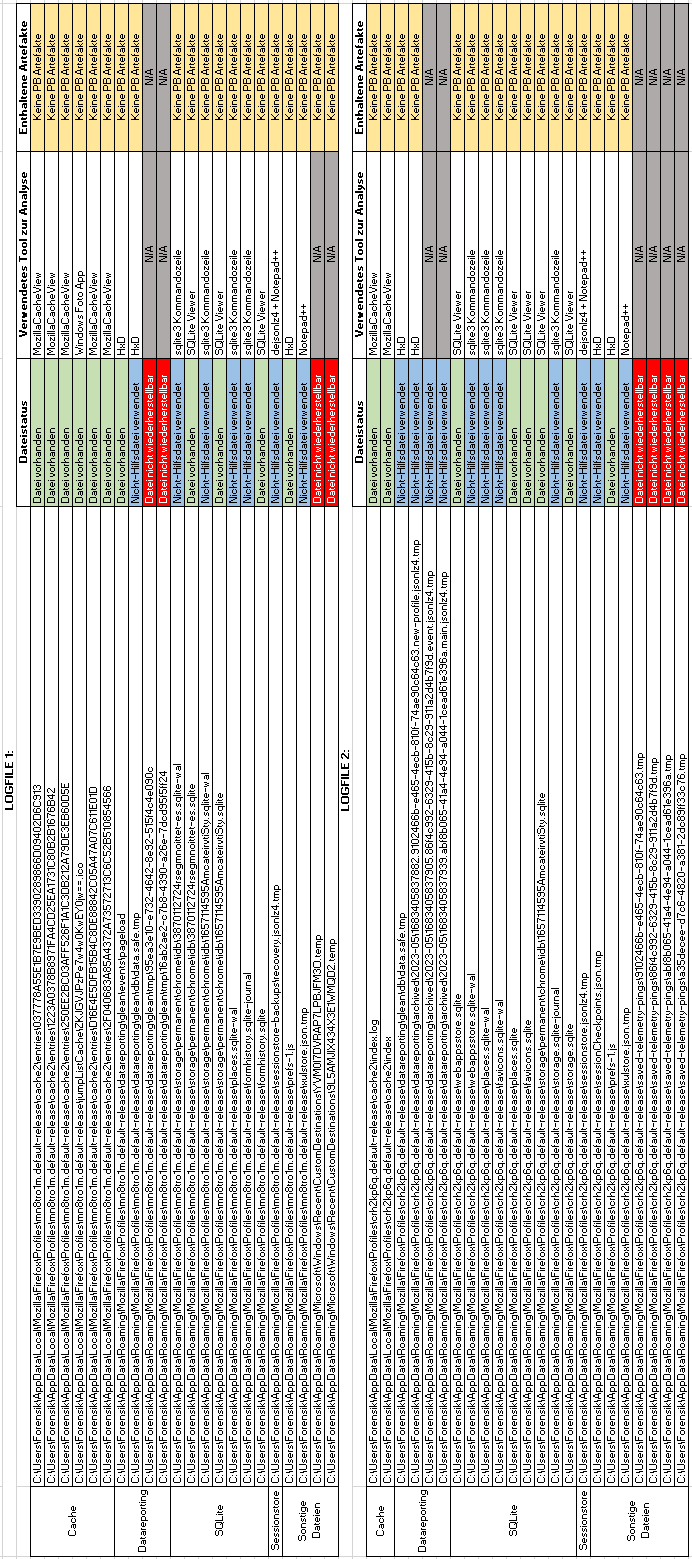
\includegraphics{bilder/firefox-all-write-operations.png}}}
%
%\end{figure}

Diese Dateien können mit dem Tool MZCacheView eingelesen werden.
Wie in Abbildung \ref{img:mzcacheview} gezeigt, konnten im Firefox Cache-Ordner des Festplatten-Images vom zweiten Snapshot drei JSON Dateien identifiziert werden. Dabei handelt es sich um Zertifikatsdateien, die von der \textit{One Certificate Revocation List} stammen, ein Mechanismus von Firefox zur Überprüfung von Zertifikaten. In keinem der Zertifikate konnten mit HxD private Browsing Artefakte oder besuchte Seiten gefunden werden. \cite{TechSupportGuy.05.06.2023}
Weiterhin befindet sich im Cache das HTML-Dokument der Firefox Datenschutzseite, welche sich beim ersten Start des Browsers automatisch öffnete, siehe Kapitel \ref{subsection:methodik-vorbereitung-browsing-szenario}
Weitere Cache Dateien konnten in keinem Festplatten-Image gefunden werden.
\begin{figure}[h!]
	\resizebox{\linewidth}{!}{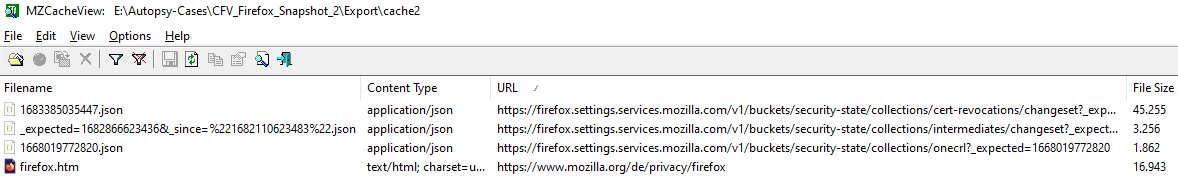
\includegraphics{bilder/firefox-cache.png}}
	\caption{MZCacheView eingelesene Firefox Cache-Dateien}
	\label{img:mzcacheview}
\end{figure}
Die Indexdatei \texttt{$\backslash$cache2$\backslash$index} dient als Datenbank im Cache. Sie ermöglicht es dem Firefox-Browser, schnell auf die zwischengespeicherten Ressourcen zuzugreifen und diese effizient zu verwalten. In diese Datei wurde beim Schließen des Browsers geschrieben. Sowohl mit HxD als auch dem Tool FirefoxCache2 konnten keine PB Artefakte identifiziert werden.

Schließlich enthält die Datei \texttt{$\backslash$jumpListCache$\backslash$ZKJGVJPzPe7w4w0KwEY0jw==.ico} ein $64x64$ Pixel großes Mozilla Logo. Dieses Logo ist keinem Schritt des Browsing Szenarios zuzuordnen.


\paragraph*{Datareporting}
Dateien im Ordner \texttt{$\backslash$datareporting$\backslash$glean$\backslash$db} sind Teil des Glean-Systems, das für die Sammlung von Telemetriedaten und deren Übermittlung an Mozilla verwendet wird. \cite{GitHub.05.06.2023}
Die Datei \texttt{data.safe.bin} enthält verschlüsselte und anonyme Informationen über die Nutzung des Browsers. In HxD konnten keine keine PB Artefakte gefunden werden. 

Dateien im Format \texttt{$\backslash$datareporting$\backslash$glean$\backslash$db$\backslash$<Profilname>.new-profile.jsonlz4} speichern Informationen über das Firefox-Profil, das von Glean verwendet wird. In diese Dateien wurde erst nach dem Browsing-Szanrio, beim Schließen des Browser geschrieben. Diese Dateien im proprietären \textit{jsonlz4}-Format lassen sich mit dem Tool dejsonlz4 dekomprimieren. Die entstandene JSON Datei wurde mit dem Notepad++ JSON Plugin untersucht. Dabei konnten keine PB Artefakte gefunden werden.

\paragraph*{Sessionstore}
Die Datei \texttt{$\backslash$sessionstore-backups$\backslash$recovery.jsonlz4} enthält eine Sicherungskopie der vorherigen Sitzung. Sie wird erstellt, wenn der Firefox-Browser nach einem Absturz oder einem unerwarteten Beenden neu gestartet wird. 
Jefferson Scher entwickelte das Online-Tool \textit{Session History Scrounger for Firefox} zur Analyse dieser ``Sessionstore-Backup`` Dateien. \cite{JeffersonScher.29.11.2020}
Wie Abbildung \ref{img:firefox-session-history-scrounger} gezeigt, enthielt die Datei sowohl im Festplatten-Image 2 (Logfile 1) und 3 (Logfile 2) nur die automatisch geöffnete Seite der Firefox Datenschutzhinweise.
\begin{figure}[h!]
	\resizebox{\linewidth}{!}{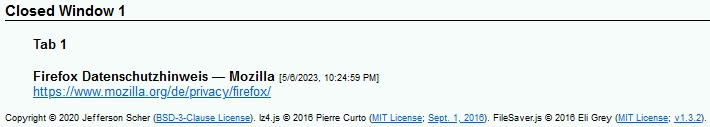
\includegraphics{bilder/firefox-sessionstore.png}}
	\caption{Firefox Sitzungsdatei \texttt{recovery.jsonlz4} geöffnet mit dem ``Session History Scrounger for Firefox``}
	\label{img:firefox-session-history-scrounger}
\end{figure}

\paragraph*{Sonstige Dateien}
In der Datei \texttt{prefs-1.js} werden benutzerspezifische Einstellungen und Konfigurationen für den Firefox-Browser gespeichert. Die Datei enthält Präferenzen des Benutzers in Form von JavaScript-Objekten. Es konnten in den Dateien beider Logfiles mit HxD keine PB Artefakte gefunden werden. 
Schließlich speichert die Datei \texttt{xulstore.json} benutzerspezifische Anpassungen und Konfigurationen des Firefox-Browsers. In der Datei konnten in den Festplatten-Images beider Logfiles mit Notepad++ keine PB Artefakte gefunden werden. \cite{mozillazine.29.12.2022}

\subsubsection*{SQLite Datenbänke}
\label{appendix:firefox-sqlite}
Wie in Kapitel \ref{subsection:methodik-datenanalyse-commonlocations} erwähnt, werden SQLite Datenbanken als Datenstrukturen für Nutzerdaten detaillierter und getrennt von den Schreiboperationen der Process Logfiles untersucht. Mithilfe der Process Monitor Logfiles wurden zunächst die in Tabelle \ref{tab:firefox-sqlite-dbs-explained} dargestellten SQLite-Datenbanken für Firefox identifiziert:
\begin{table}[h!]
\caption{Veränderte Firefox SQLite-Datenbänke und deren Verwendungszwecke}
\label{tab:firefox-sqlite-dbs-explained}
\resizebox{\linewidth}{!}{
\begin{tabular}{|l|l|lll}
\cline{1-2}
\textbf{Datenbank}                        & \textbf{Gespeicherte Daten \cite{GitHub.08.04.2019}}                                                                                             &  &  &  \\ \cline{1-2}
\textit{places.sqlite}                    & Informationen über Lesezeichen und Verlauf. Zu jeder besuchten Webseite: URL, Seitentitel, Zeitstempel des Besuchs etc.  &  &  &  \\ \cline{1-2}
\textit{cookies.sqlite}                   & Von besuchten Webseiten verwendete Cookies.                                                                              &  &  &  \\ \cline{1-2}
\textit{storage.sqlite}                   & Diverse Webdaten, z. B. Indexed-Datenbanken, Offline-Cache-Daten und andere lokale Speicherinformationen.                &  &  &  \\ \cline{1-2}
\textit{favicons.sqlite}                  & Enhtält Favicons (kleine Symbole in der Adressleiste) um besuchte Webseiten visuell zu identifizieren.                   &  &  &  \\ \cline{1-2}
\textit{webappsstore.sqlite}              & Speichert Informationen über installierte Webanwendungen im Firefox-Browser, z.B. Berechtigungen und Einstellungen.      &  &  &  \\ \cline{1-2}
\textit{1657114595AmcateirvtiSty.sqlite}  & Datenspeicher für Activity Stream, eine personalisierte Übersicht über Browser-Aktivitäten beim Öffnen eines neuen Tabs. &  &  &  \\ \cline{1-2}
\textit{3870112724rsegmnoittet-es.sqlite} & Datenspeicher für Remote Settings, eine zentrale Verwaltung von benutzerspezifischen Browsereinstellungen.               &  &  &  \\ \cline{1-2}
\end{tabular}
}
\end{table}

Entsprechend der Methodik in Kapitel \ref{subsubsection:methodik-datenanalyse-commonlocations-sqlitedbs} wurde jede SQLite-Datenbank aus allen vier Snapshots extrahiert und verglichen.
Die Ergebnisse sind in Tabelle \ref{tab:firefox-veraenderte-sqlitedbs} dargestellt.

\begin{table}[h!]
\centering
\caption{Veränderung der Firefox SQLite-Datenbänke während der Versuchsdurchführung}
\label{tab:firefox-veraenderte-sqlitedbs}  
\resizebox{\linewidth}{!}{
\begin{tabular}{|l|c|cc|cc|cc|}
\hline
\multicolumn{1}{|c|}{}                                     &                                                                                                    & \multicolumn{2}{c|}{\textbf{\begin{tabular}[c]{@{}c@{}}Nach Browsing Szenario, \\ Browser geöffnet (S2)\end{tabular}}}                                                                                                                              & \multicolumn{2}{c|}{\textbf{\begin{tabular}[c]{@{}c@{}}Nach Browsing Szenario, \\ Browser geschlossen (S3)\end{tabular}}}                                                                                                            & \multicolumn{2}{c|}{\textbf{\begin{tabular}[c]{@{}c@{}}VM \\ heruntergefahren (S4)\end{tabular}}} \\ \cline{3-8} 
\multicolumn{1}{|c|}{\multirow{-2}{*}{\textbf{Dateiname}}} & \multirow{-2}{*}{\textbf{\begin{tabular}[c]{@{}c@{}}Vor Browsing \\ Szenario\\ (S1)\end{tabular}}} & \multicolumn{1}{c|}{\textbf{Vor WAL}}                                                                                                      & \textbf{Nach WAL}                                                                                      & \multicolumn{1}{c|}{\textbf{Vor WAL}}                                                                                       & \textbf{Nach WAL}                                                                                      & \multicolumn{1}{c|}{\textbf{Vor WAL}}                     & \textbf{Nach WAL}                     \\ \hline
places.sqlite                                              & \cellcolor[HTML]{C0C0C0}N/A                                                                        & \multicolumn{1}{c|}{\cellcolor[HTML]{F56B00}\begin{tabular}[c]{@{}c@{}}Initialisiert \\ (Datenschutz-Seite)\end{tabular}}                  & \cellcolor[HTML]{FE996B}                                                                               & \multicolumn{1}{c|}{\cellcolor[HTML]{F56B00}Indizes aktualisiert}                                                           & \cellcolor[HTML]{FE996B}                                                                               & \multicolumn{2}{c|}{\cellcolor[HTML]{FE996B}}                                                     \\ \cline{1-3} \cline{5-5}
cookies.sqlite                                             & \cellcolor[HTML]{C0C0C0}N/A                                                                        & \multicolumn{1}{c|}{\cellcolor[HTML]{FFCE93}}                                                                                              & \cellcolor[HTML]{FE996B}                                                                               & \multicolumn{1}{c|}{\cellcolor[HTML]{FE996B}}                                                                               & \cellcolor[HTML]{FE996B}                                                                               & \multicolumn{2}{c|}{\cellcolor[HTML]{FE996B}}                                                     \\ \cline{1-2}
storage.sqlite                                             & \cellcolor[HTML]{C0C0C0}N/A                                                                        & \multicolumn{1}{c|}{\cellcolor[HTML]{FFCE93}}                                                                                              & \cellcolor[HTML]{FE996B}                                                                               & \multicolumn{1}{c|}{\cellcolor[HTML]{FE996B}}                                                                               & \cellcolor[HTML]{FE996B}                                                                               & \multicolumn{2}{c|}{\cellcolor[HTML]{FE996B}}                                                     \\ \cline{1-2}
favicons.sqlite                                            & \cellcolor[HTML]{C0C0C0}N/A                                                                        & \multicolumn{1}{c|}{\multirow{-3}{*}{\cellcolor[HTML]{FFCE93}\begin{tabular}[c]{@{}c@{}}Initialisiert \\ (Nur Spaltennamen)\end{tabular}}} & \multirow{-4}{*}{\cellcolor[HTML]{FE996B}\begin{tabular}[c]{@{}c@{}}keine \\ Veränderung\end{tabular}} & \multicolumn{1}{c|}{\multirow{-3}{*}{\cellcolor[HTML]{FE996B}\begin{tabular}[c]{@{}c@{}}keine \\ Veränderung\end{tabular}}} & \cellcolor[HTML]{FE996B}                                                                               & \multicolumn{2}{c|}{\cellcolor[HTML]{FE996B}}                                                     \\ \cline{1-5}
webappsstore.sqlite                                        & \cellcolor[HTML]{C0C0C0}N/A                                                                        & \multicolumn{1}{c|}{\cellcolor[HTML]{C0C0C0}N/A}                                                                                           & \cellcolor[HTML]{C0C0C0}N/A                                                                            & \multicolumn{1}{c|}{\cellcolor[HTML]{FFCE93}\begin{tabular}[c]{@{}c@{}}Initialisiert \\ (Nur Spaltennamen)\end{tabular}}    & \cellcolor[HTML]{FE996B}                                                                               & \multicolumn{2}{c|}{\cellcolor[HTML]{FE996B}}                                                     \\ \cline{1-5}
formhistory.sqlite                                         & \cellcolor[HTML]{C0C0C0}N/A                                                                        & \multicolumn{1}{c|}{\cellcolor[HTML]{FFCE93}\begin{tabular}[c]{@{}c@{}}Initialisiert \\ (Nur Spaltennamen)\end{tabular}}                   & \cellcolor[HTML]{FE996B}                                                                               & \multicolumn{1}{c|}{\cellcolor[HTML]{FE996B}keine Veränderung}                                                              & \cellcolor[HTML]{FE996B}                                                                               & \multicolumn{2}{c|}{\cellcolor[HTML]{FE996B}}                                                     \\ \cline{1-3} \cline{5-5}
1657114595AmcateirvtiSty.sqlite                            & \cellcolor[HTML]{C0C0C0}N/A                                                                        & \multicolumn{1}{c|}{\cellcolor[HTML]{CE6301}\begin{tabular}[c]{@{}c@{}}Initialisiert \\ (``origin``: ``chrome``)\end{tabular}}                 & \cellcolor[HTML]{FE996B}                                                                               & \multicolumn{1}{c|}{\cellcolor[HTML]{F56B00}\begin{tabular}[c]{@{}c@{}}Binärdaten, \\ keine PB Artefakte\end{tabular}}      & \cellcolor[HTML]{FE996B}                                                                               & \multicolumn{2}{c|}{\cellcolor[HTML]{FE996B}}                                                     \\ \cline{1-3} \cline{5-5}
3870112724rsegmnoittet-es.sqlite                           & \cellcolor[HTML]{C0C0C0}N/A                                                                        & \multicolumn{1}{c|}{\cellcolor[HTML]{CE6301}\begin{tabular}[c]{@{}c@{}}Initialisiert \\ (``origin``: ``chrome``)\end{tabular}}                 & \multirow{-3}{*}{\cellcolor[HTML]{FE996B}\begin{tabular}[c]{@{}c@{}}keine \\ Veränderung\end{tabular}} & \multicolumn{1}{c|}{\cellcolor[HTML]{FE996B}keine Veränderung}                                                              & \multirow{-12}{*}{\cellcolor[HTML]{FE996B}\begin{tabular}[c]{@{}c@{}}keine \\ Veränderung\end{tabular}} & \multicolumn{2}{c|}{\multirow{-12}{*}{\cellcolor[HTML]{FE996B}keine Veränderung}}                  \\ \hline
\end{tabular}
}
\end{table}

Unmittelbar nach der Installation von Firefox (Snapshot 1) existierte noch keine der SQLite-Dateien.
Nach dem Browsing Szenario (Snapshot 2) wurden alle SQLite-Datenbanken außer \texttt{webappsstore.sqlite} 
initialisiert. Dabei wurden in \texttt{places.sqlite} die automatisch im normalen Modus geöffnete Firefoxseite der Datenschutzhinweise eingetragen. 
Die restlichen Datenbanken wurden leer initialisiert, nur die Spaltennamen wurden definiert.
Der Inhalt aller initialisierten Datenbanken blieb nach Durchführung von PRAGMA WAL Checkpoints unverändert.
Nach Schließen des Browsers (Snapshot 3) wurden in \texttt{places.sqlite} die Indizes der eingetragenen Seiten aktualisiert. Die SQLite-Datenbank \texttt{1657114595AmcateirvtiSty.sqlite} erhielt ein binäres Datenobjekt als Eintrag. Bei der Untersuchung mit HxD konnten keine Artefakte gefunden werden. Weiterhin wurde \texttt{webappsstore.sqlite} leer initialisiert. Die restlichen Daten blieben im Vergleich mit Snapshot 2 unverändert. Ebenfalls veränderte sich nicht der Inhalt nach Durchführung von PRAGMA WAL Checkpoints.
Sowohl nachdem die VM herunterfahren wurde, (Snapshot 4) als auch nach Durchführung der PRAGMA WAL Checkpoints, entstanden keine Änderungen in den SQLite Datenbanken.	
Somit wurden in den SQLite Datenbanken von Firefox keine zurückverfolgbaren PB Artefakte im privaten Modus hinterlassen.

\subsubsection*{Zusammenfassung Firefox Common Locations}
Mithilfe der Process Monitor Logfiles wurde festgestellt, dass sowohl während des Browsing Szenarios (Logfile 1) als auch danach (Logfile 2) Inhalte in Dateien geschrieben wurden. Wie in Abbildung \ref{chart:firefox-writefile-logfile1v2} dargestellt, gab es mit Ausnahme der Datareporting Dateien in Logfile 1 stets mehr oder gleich viele Schreiboperationen wie in Logfile 2. Keine der Schreiboperation hinterließ Private Browsing Artefakte.

\begin{figure}[h!]
	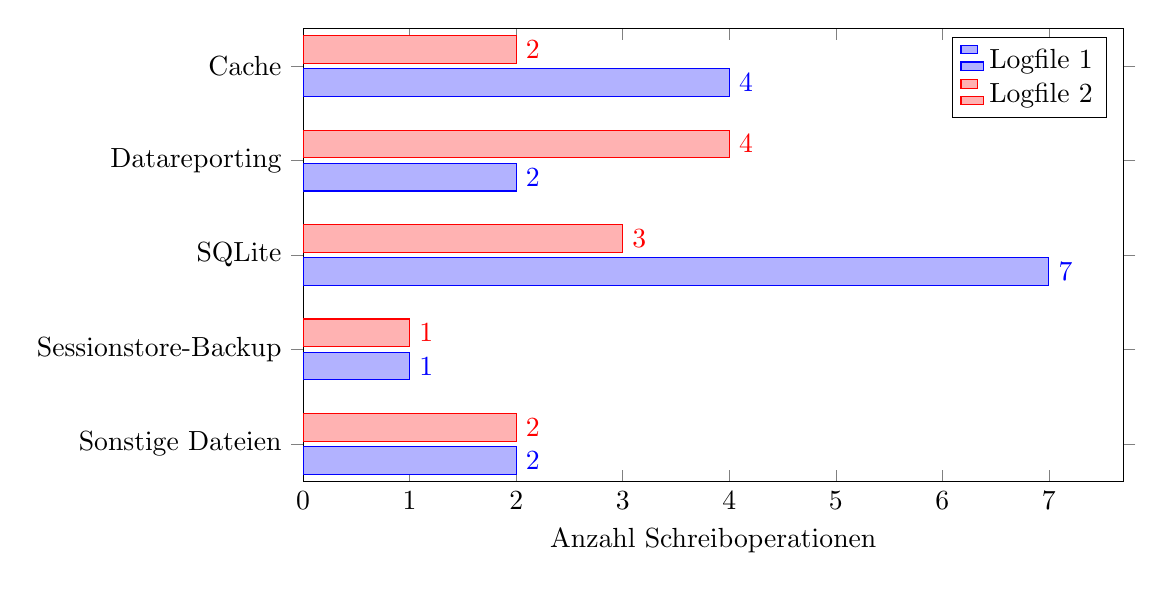
\begin{tikzpicture}
	\begin{axis}[
	xbar, 
	xmin=0,
	width=12cm, 
	height=12cm, 
	xlabel={Anzahl Schreiboperationen},
	y=1.2cm,
	%					0  					1			   2 		  3			 4
	%yticklabels={Sonstige Dateien, Sessionstore-Backup, SQLite, Datareporting, Cache},
	%ytick=data,
	symbolic y coords={Sonstige Dateien,Sessionstore-Backup,SQLite,Datareporting,Cache},
	ytick=data,
	%symbolic y coords={Sonstige-Dateien,Sessionstore-Backup,SQLite,Datareporting,Cache},
	%ytick=data,
	nodes near coords, nodes near coords align={horizontal},
	]
	\addplot coordinates {(2,Sonstige Dateien) (1,Sessionstore-Backup) (7,SQLite) (2,Datareporting) (4,Cache)};
	\addplot coordinates {(2,Sonstige Dateien) (1,Sessionstore-Backup) (3,SQLite) (4,Datareporting) (2,Cache)};
	
	\legend{Logfile 1, Logfile 2}
	\end{axis}
	\end{tikzpicture}
	\caption{Firefox Anzahl Schreiboperationen Logfile 1 vs Logfile 2, geordnet nach Kategorie}
	\label{chart:firefox-writefile-logfile1v2}
\end{figure}

%Literatur:
%	o no traces were found in “common locations” \cite{Montasari.2015}
%		>  “places.sqlite”, “webappsstore. sqlite”, “sessionstore.bak”, “search.json” and “nssckbi.dll”
%	o	Safebrowsing: Alle Dateien in /safebrowsing-updating/ nicht relevant. Dort nur .vlpset und .sbstore Dateien. Speichern 256-Bit Hash von URLs, die auf SafeSearch Blacklist stehen 
%	o	Cache-Dateien: drei Caches: startupCache, jumpListCache (beide enthalten Binärdateien ohne Browsing Artefakte) und cache2 (können mit MozillaCacheView untersucht werden, enthalten keine Browsing Artefakte)
%	o	SQLite Datenbanken: Sqlite Dateien erst ohne WAL Dateien untersuchen, Danach mit sqlite3 Konsole: WAL in Datenbank schreiben mit: PRAGMA wal\_checkpoint; places.sqlite besonders relevant, da dort Browser in public Modus Browsing URLs verwaltet (Am besten hier vergleich mit Public Browsing machen)	
%		> \cite{Fayyad.2021} for Mozilla Firefox, 7 database files were recovered: cookies.sqlite-shm, places.sqlite-shm, prefs.js etc.
%		> \cite{Muir.2019} The two SQLite databases used by Firefox to track cookies and history (cookies.sqlite und places.sqlite) were both recoverable from the file system after deletion	
%		Ergebnisse stehen im Gegensatz zu \cite{Hedberg.2013} :
%			o	Chrome und Firefox: Einträge in places.sqlite + history.sqlite DB gefunden während PB! (Noch aktuell??)
%		Sonderfall: SQlite DB-Crash \cite{Hedberg.2013}
%			> WAL Files/Journal Files bei Crash gefunden -> Kann genutzt werden um zu beweisen, dass privater Browser genutzt wurde
%			> Daher: WAL Rollback mit sqlite3	
%	o	Jsonlz4 \& balkz4: Enthalten komprimierte Firefox-Sessions, jsonlz4 Dateien können mit Tool ``entkomprimiert`` werden: https://www.jeffersonscher.com/ffu/scrounger.html

\subsection{Uncommon Locations}
\label{subsection:appendix-firefox-uncommon-locations}

\subsubsection*{Analyse mit Autopsy - Kategorisierte Dateien}
\label{subsubsection:appendix-firefox-uncommon-locations-autopsy}

Beim Vergleich der Festplattenabbilder wurde festgestellt, dass ein Festplatten-Image stets die kategoriesierten Dateien des Festplatten-Images des vorherigen Snapshots enthielt. Somit enthält das Festplatten-Image von Snapshot 4 alle kategorisierten Dateien der vorherigen Snapshots.

\paragraph*{Web Bookmarks}
Bereits vor Durchführung des Browsing Szenarios enthielt Firefox im ersten Snapshot die in Abbildung \ref{img:firefox-web-bookmarks} dargestellte Bing Startseite als gespeichertes Leesezeichen. In den restlichen Snapshots 2 -- 4 blieb diese Kategorie unverändert.
\begin{figure}[h!]
	\centerline{\resizebox{\linewidth}{!}{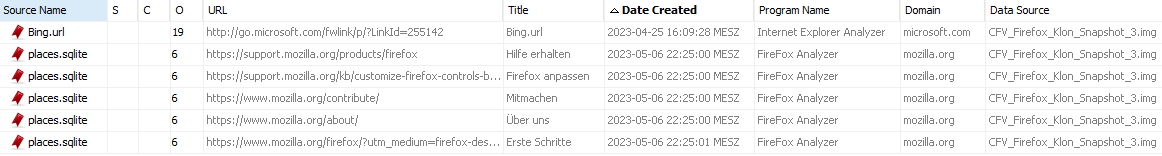
\includegraphics{bilder/cfv_firefox_autopsy_web_bookmarks.png}}}
	\caption{Firefox: Von Autopsy als ``Web Bookmarks`` kategorisierte Dateien}
	\label{img:firefox-web-bookmarks}  
\end{figure}

\paragraph*{Web Cookies}
Die Kategorie ``Web Cookies`` enthält bereits vor Beginn des Browsing Szenarios zehn in Abbildung \ref{img:firefox-web-cookies} gezeigte Cookie-Einträge in der Datei \texttt{WebCacheV01.dat}. Dabei handelt es sich um eine Datenbank des Microsoft Edge Browsers zur Speicherung von Nutzerdaten. Diese Datei verhält sich ähnlich wie die in diesem Versuch relevanten SQLite-Dateien. Bei den Einträgen handelt es sich um Cookies für Bing und die Outlook Webseite, obwohl diese Seiten nie in Microsoft Edge geöffnet wurden. In den Snapshots 2 -- 4 kamen keine weiteren Einträge in dieser Kategorie hinzu.
\begin{figure}[h!]
	\centerline{\resizebox{\linewidth}{!}{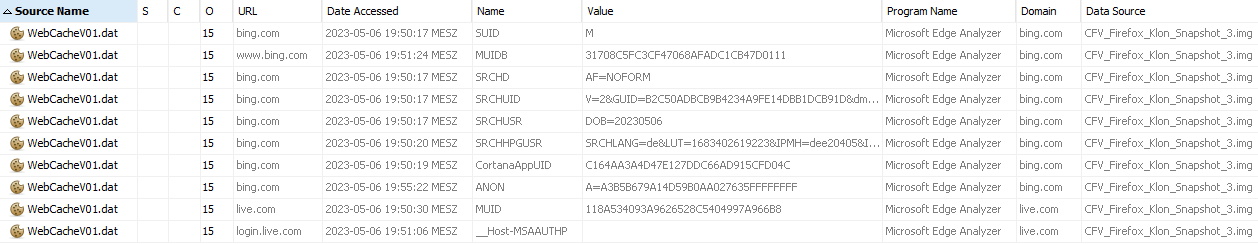
\includegraphics{bilder/cfv_firefox_autopsy_web_cookies.png}}}
	\caption{Firefox: Von Autopsy als ``Web Cookies`` kategorisierte Dateien}
	\label{img:firefox-web-cookies}  
\end{figure}

\paragraph*{Web History}
Die Kategorie ``Web History`` listet alle Dateien mit gespeichertem Suchverlauf auf. Vor Beginn des Browsing Szenarios (Snapshot 1) enthält die Kategorie zwei Einträge zur Outlook Webseite in der Datei \texttt{WebCacheV01.dat}. Nach Durchführung des Browsing Szenarios (Snapshot 2) wurde ein Eintrag in der \texttt{places.sqlite} Datenbank hinzugefügt. Dabei handelt es sich um die automatisch im normalen Browsingmodus geöffnete Firefox-Standardseite über Datenschutzhinweise. Dies deckt sich mit den Beobachtungen der Common Locations in Anhang \ref{subsection:appendix-firefox-common-locations}. Darüber hinaus enthält dieser Snapshot für die Datei \texttt{WebCacheV01.dat} den Eintrag \texttt{file:///Z:/Logfile\_1}. Dabei handelt es sich um das Process Monitor Logfile, das gemäß Methodik in Kapitel \ref{section:methodik-vorbereitung} über den gemeinsamen VM-Ordner zum Analyse-Rechner transportiert wurde. Ergänzt wird die Kategorie in Snapshot 3 durch den Eintrag \texttt{file:///Z:/Logfile\_2}, dem zweiten Process Monitor Logfile. In Snapshot 4 werden in dieser Katgeorie keine neuen Dateien erfasst. Die kategorisierten Dateien sind in Abbildung \ref{img:firefox-web-history} dargestellt.
\begin{figure}[h!]
	\centerline{\resizebox{\linewidth}{!}{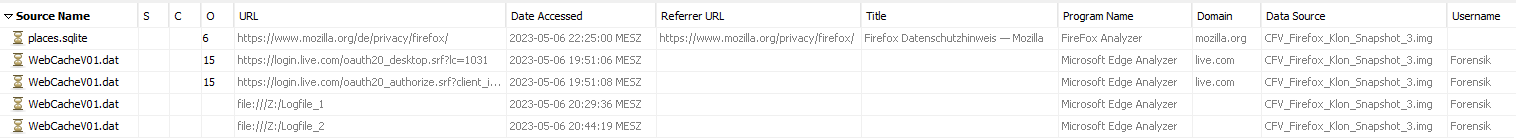
\includegraphics{bilder/cfv_firefox_autopsy_web_history.png}}}
	\caption{Firefox: Von Autopsy als ``Web History`` kategorisierte Dateien}
	\label{img:firefox-web-history}  
\end{figure}

\paragraph*{Web Categories}
Diese Kategorie klassifiziert im Speicherabbild gefundene Browsing Artefakte nach Inhalt.
Vor Beginn des Browsing Szenarios (Snapshot 1) werden hier bereits zwei in Abbildung \ref{img:firefox-web-categories} dargestellte Einträge aufgelistet. Der Eintrag \texttt{bing.com} wird als ``Suchmaschine`` klassifiziert und \texttt{live.com} als ``Web-Email``.
Wie oben erwähnt, wurden beide Seiten nie aufgerufen. Es gab keine zusätzlichen Einträge in dieser Kategorie in den Snapshots 2 bis 4.
\begin{figure}[h!]
	\centerline{\resizebox{\linewidth}{!}{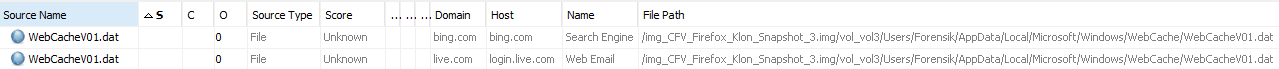
\includegraphics{bilder/cfv_firefox_autopsy_web_categories.png}}}
	\caption{Firefox: Von Autopsy als ``Web Categories`` kategorisierte Dateien}
	\label{img:firefox-web-categories}  
\end{figure}

Somit wurden in allen Kategorien ausschließlich Browsing Artefakte des Edge Browsers in der Datei \texttt{WebCacheV01.dat} gefunden, sowie ein Eintrag in der Firefox SQLite Datenbank \texttt{places.sqlite}. In keiner der Kategorien konnten private Browsing Artefakte identifiziert werden. Die von Autopsy erkannte Firefox-Standardseite deckt sich mit den Ergebnissen der Common Locations. Die aufgelisteten Einträge in der Datei \texttt{WebCacheV01.dat} sind nicht auf Schritte des Browsing Szenarios zurückzuführen. Die Einträge sind bereits im ersten Snapshot enthalten, obwohl vor Beginn des Browsing Szenarios keine Browseraktivitäten durchgeführt wurden. Weiterhin enthält diese Datei Einträge über die Process Monitor Logfiles, welche über einen gemeinsamen VM-Ordner zum Rechner transportiert wurde, auf dem die virtuelle Maschine läuft.

%Literatur:
%	o	Autopsy Keywortsuche: 
%		>	In alles Snapshots ergebnislos (keine Keyword-Hits
%		-->	In Literatur: Autoren fanden Ergebnisse in pagefile.sys 
%			> Autopsy: websites and some of the keywords found in hidden file called “pagefile.sys” \cite{Mahlous.2020}
%			o \cite{Montasari.2015} traces were found in: 
%				> However, on investigating the “pagefile.sys”, some entries were discovered
%				> Using the “data carving” technique, profile picture was recovered
%			o \cite{Said.2011} 
%				> Examining pagefile.sys showed some positive hits 			
%		--> Evtl. hier zeigen, was gefunden werden kann, wenn RAM reduziert
%		--> Aber auf Problem hinweisen, dass gefundener String in pagefile nicht direkt Browser zugeordnet werden kann
%		> \cite{Gabet.2018}	Firefox only produced three recoverable artefacts as reported by both tools (FTK, Autopsy) --> Artefakte werden nicht genannt!
%		> \cite{Muir.2019} Autopsy Keyword Suche nach Suchbegriffen: unallocated space
%		> Autopsy Carving Module (\$Carved): \cite{Muir.2019}
%			•	When searching for the string ’clot’ from the browsing protocol, six .dll, .edb and .reg files were discovered in unallocated space.
%			•	Further searching of unallocated space uncovered references to the Tor installation directory and the obfs4 bridging IP addresses
%			•	browsing data found in NTUSER.DAT was also replicated in unallocated space.
%	o	Autopsy PlugIns:
%		>	*** TODO: Hier Liste mit PlugIns ***

\subsection*{Registry}
\label{subsection:appendix-firefox-registry}

\subsubsection*{Process Monitor SetValue Operations}
\label{subsubsection:appendix-firefox-registry-processmonitorsetvalue}
Als Teil der Common Locations werden für Firefox alle Registry ``SetValue`` Schreiboperationen der beiden Process Monitor Logfiles untersucht.

In beiden Logfiles wurden zwei Kategorien von Registry Keys geschrieben: \textit{PreXULSkeletonUISettings} und \textit{Business Activity Monitoring}. In Abbildung \ref{chart:firefox-registy-css-vs-bam} ist der Anteil der Schreiboperationen je Kategorie für beide Logfiles gezeigt.
\begin{figure}[h!]
	\resizebox{\linewidth}{!}{
	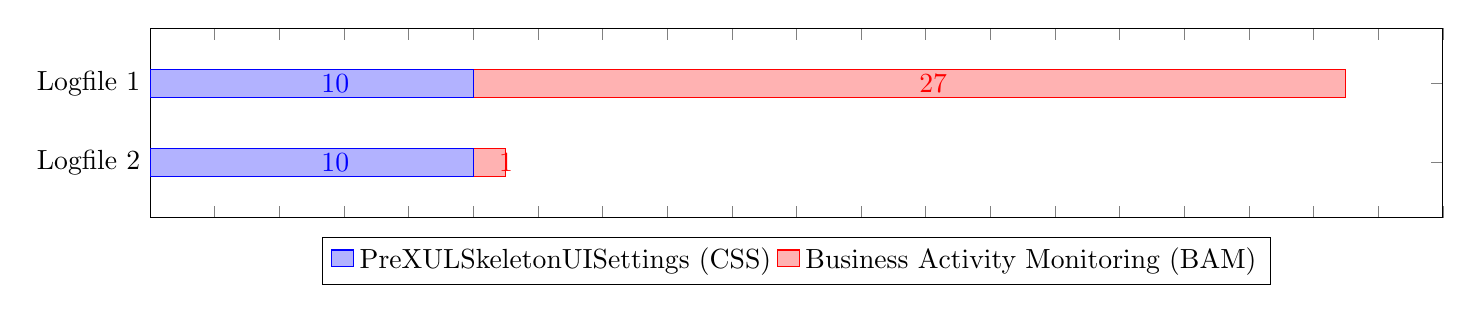
\begin{tikzpicture}
		\begin{axis}[
		xbar stacked,
		width=18cm, 
		height=12cm, 
%		ylabel style={align=center}, ylabel=RAM-Dump 1,
		y=1cm,
		enlarge y limits={abs=2*\pgfplotbarwidth},
		symbolic y coords={Logfile 2,Logfile 1},
		ytick=data,
		xticklabels={,,},
        xmin = 0,
        xmax = 40,
		nodes near coords, 
		nodes near coords align={horizontal},
		legend style={
			at={(0.5,-0.1)},
			anchor=north
		},
		legend columns=2,
		scaled x ticks=false
		]
			\addplot coordinates {
			(10,Logfile 2) (10,Logfile 1)
			};
			\addplot coordinates {
			(1,Logfile 2) (27,Logfile 1)
			};
			\legend{PreXULSkeletonUISettings (CSS), Business Activity Monitoring (BAM)}
		\end{axis}
	\end{tikzpicture}
	}	
	\caption{Firefox Registry ``SetValue`` Operationen in den Process Monitor Logfiles 1 und 2}
	\label{chart:firefox-registy-css-vs-bam}
\end{figure}

%\begin{figure}[h!]
%	\centerline{\resizebox{\linewidth}{!}{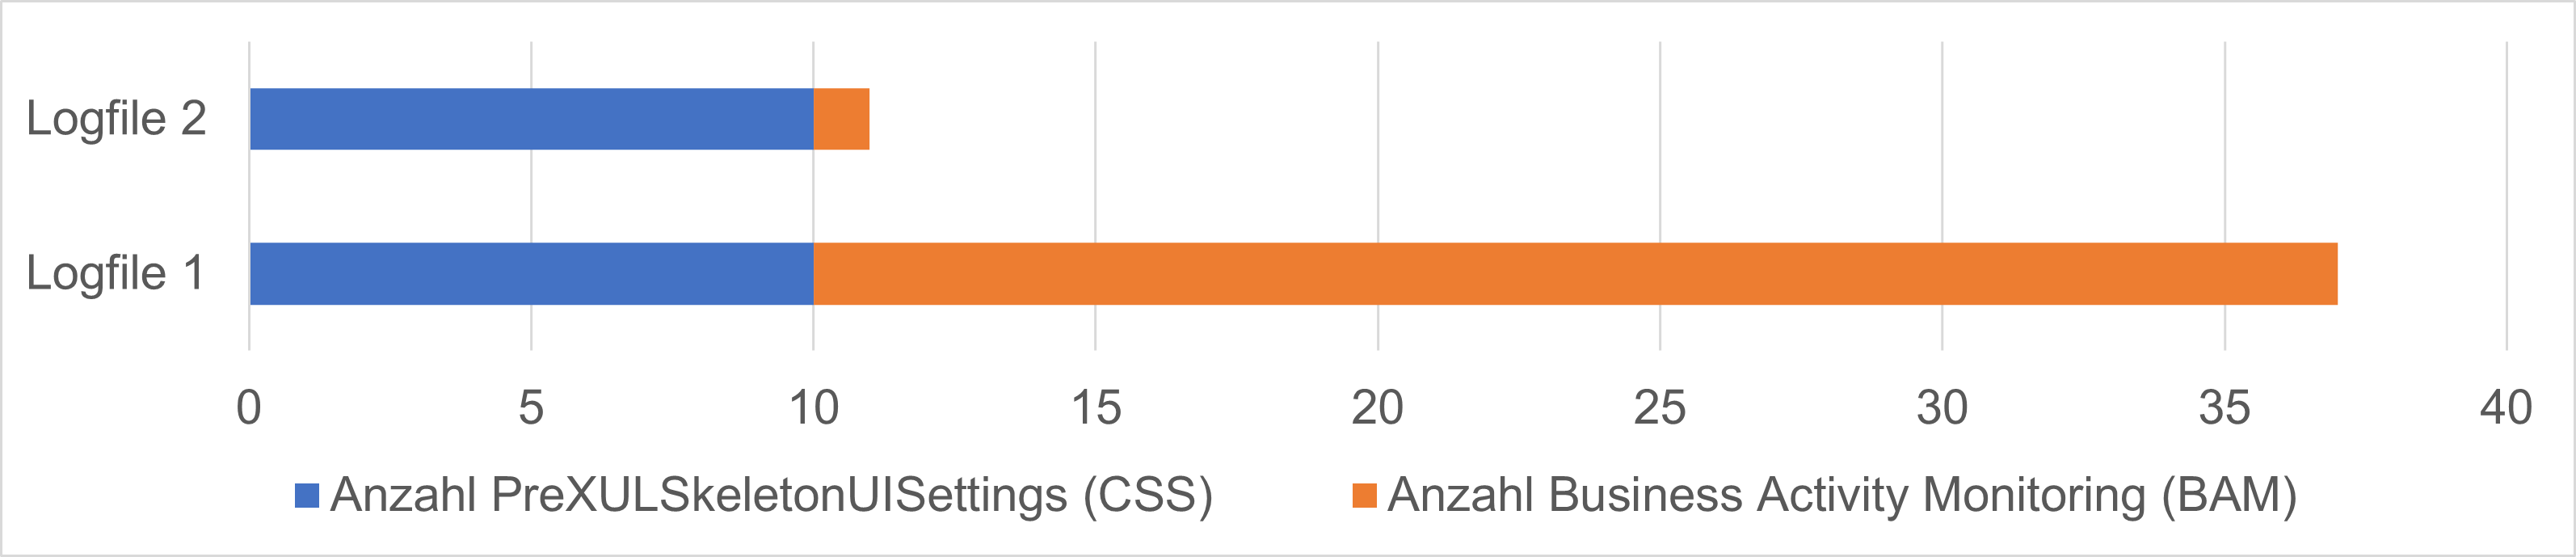
\includegraphics{bilder/firefox-registry-stacked-bar-chart.png}}}
%	\label{chart:final-criteria}  
%	\caption{Comparison of found PB artifacts between RAM Dumps}
%\end{figure}

\paragraph*{PreXULSkeletonUISettings}
Der \textit{PreXULSkeletonUISettings} Registry Key enthält Einstellungen für die Benutzeroberfläche (UI) des Firefox-Browsers, insbesondere für das sogenannte \textit{Skeleton UI}, eine vereinfachte Benutzeroberfläche, die während des Ladens des Browsers angezeigt wird, bevor die vollständige Benutzeroberfläche geladen ist. 
PreXULSkeletonUISettings Registry Keys haben das Format \texttt{HKCU$\backslash$SOFTWARE$\backslash$Mozilla$\backslash$Firefox$\backslash$\\PreXULSkeletonUISettings$\backslash$<Absoluter Firefox Installationspfad>$\backslash$firefox.exe|<Skeleton UI Setting>}.
Somit enthält der Key den absoluten Installationspfad von Firefox gefolgt von einer Skeleton UI Einstellung. Nachfolgend sind alle möglichen UI Einstellungen aufgelistet, gefolgt vom Datentyp des Keys. \cite{Mills.2021}
\begin{itemize}
	\item ScreenX (DWORD)
	\item ScreenY (DWORD)
	\item Width (DWORD)
	\item Height (DWORD)
	\item Maximized (DWORD)
	\item Flags (DWORD)
	\item CssToDevPixelScaling (REG\_BINARY)
	\item UrlbarCSSSpan (REG\_BINARY)
	\item SearchbarCSSSpan (REG\_BINARY)
	\item SpringsCSSSpan (REG\_BINARY)
\end{itemize}
Somit enthalten die Keys nur Daten zur Formatierung und Struktur der grafischen Oberfläche. Es wurden keine PB Artefakte geschrieben

\paragraph*{Business Activity Monitoring}
\textit{Business Activity Monitoring}, kurz \textit{BAM} ist eine weitgehend undokumentierte Windows Funktion, die im Hintergrund ausgeführte Programme steuert.
Der Registry Key hat das Format \texttt{HKLM$\backslash$System$\backslash$CurrentControlSet$\backslash$Services$\backslash$bam$\backslash$State$\backslash$\\UserSettings$\backslash$<SID>$\backslash$Device$\backslash$HarddiskVolume2$\backslash$<Absoluter Firefox Installationspfad>$\backslash$firefox.exe} und den Datentyp REG\_BINARY.
Jeder Schlüssel wird durch die Sicherheits-ID (SID) des Benutzers identifiziert.
Ein BAM Registry Key schreibt für alle ausgeführten Programme --- hier Firefox --- den Zeitstempel der letzten Ausführung.
PB Artefakte sind dabei nicht enthalten. \cite{MandiOhlinger.05.06.2023, InfoSecNotes.05.06.2023}

\subsubsection*{Stringsuche in Registry Hives}
Gemäß Methodik in Kapitel \ref{subsection:methodik-datenanalyse-registry} wird die Firefox Registry als Uncommon Location behandelt, indem über alle auf der Festplatte vorhandenen Registry Datenbanken, den Registry-Hives, eine Stringsuche durchgeführt wird, ohne die Struktur der Hives zu beachten. 
Dazu wurden sowohl die System-Hives als auch die User-Hives aus Tabelle \ref{tab:windows-registry-hives} aus jedem Festplatten-Image extrahiert und mithilfe des Registry Explorers nach PB Artefakten durchsucht.
Dabei wurde in keinem Snapshot in keinem Hive ein PB Artefakt gefunden.

%Literatur:
%	>	Auf Autor verweisen: angeblich in Shellactivities Ergebnisse. --> Nicht mehr vorhanden in aktueller Version (Verweis auf E-Mail)
%	>	Process Monitor/Regshot zeigen keine relevanten Key-Änderungen
%	> \cite{Muir.2019}: Autopsy Keyword Suche nach Suchbegriffen: Ergebnisse in \%SystemRoot\%Minidump NTUSER.DAT, ntuser.dat.LOG1 (a log of changes to NTUSER.DAT)
%	> Zentral: shellactivites Key:	NTUSER.DAT --> “shellactivities” key \cite{Muir.2019}
%	> \cite{Rochmadi.2017} Detection of registry changes helps to determine what the appropriate plugin is used to search for digital evidence using volatility memory forensic:
%	- RegQueryValue:	HKCU/Software/Microsoft/Windows/CurrentVersion/InternetSettings/Connections/DefaultConnectionSettings
%	- RegCloseValue: 	HKCU/Software/Microsoft/Windows/CurrentVersion/InternetSettings/Connections
%	- IRP\_MJ\_READ: C:/pagefile.sys


%%%%%%%%%%%%%%%%%%%%%%%%%%%%%%%%%%%%%%%%%%%%%%%%%%%%%%%%%%%%
%%%%%%%%%%%%%%%%%%%%%%%%%%%%%%%%%%%%%%%%%%%%%%%%%%%%%%%%%%%%
%%%%%%%%%%%%%%%%%%%%%%%%%%%%%%%%%%%%%%%%%%%%%%%%%%%%%%%%%%%%

\section{Ausführliche Analyse: Tor}
\subsection{Common Locations}

\subsubsection*{Process Monitor WriteFile Operations}

Bei der Versuchsdurchführung für den Tor-Browser gemäß Kapitel \ref{section:methodik-datensammlung} wurden drei Process Monitor Logfiles erstellt.
Diese Dateien enthalten alle aufgezeichneten Prozessaktivitäten während des Browsing Szenarios, nach dem Erzeugen einer ``Neuen Identität`` sowie nach Schließen des Browsers.
Tabelle \ref{tab:tor-writefile-operations} enthält alle in den Logfiles identifizierten Dateien.
Für jede Datei wurde vermerkt ob und wie sie wiederherstellbar war, mit welchem Tool die Datei analysiert wurde und ob PB Artefakte enthalten sind.
Die Dateien wurden in die Kategorien \textit{Cache}, \textit{datareporting}, und \textit{Sonstige Dateien} eingeordnet.
In keiner der identifizierten Dateien konnten PB Artefakte gefunden werden. 

Es konnten zwei Datei-Pfade identifiziert werden:
\begin{itemize}
\item[\textbf{Caches}] \texttt{C:$\backslash$Users$\backslash$Forensik$\backslash$Desktop$\backslash$Tor Browser$\backslash$Browser$\backslash$TorBrowser$\backslash$Data$\backslash$Browser$\backslash$\\Caches$\backslash$profile.default$\backslash$}
\item[\textbf{Profile.default}] \texttt{C:$\backslash$Users$\backslash$Forensik$\backslash$Desktop$\backslash$Tor Browser$\backslash$Browser$\backslash$TorBrowser$\backslash$Data$\backslash$Browser$\backslash$\\profile.default$\backslash$}
\end{itemize}
In der Tabelle sind die Dateien je nach Speicherort \textit{Caches} (Hellblau) oder \textit{Profile.default} (Dunkelblau) eingefärbt. 

Bei der Auswertung der Process Monitor Logfiles wurde festgestellt, dass alle Schreibopertationen von ``firefox.exe`` Prozessen durchgeführt wurde, nicht ``tor.exe``. Obwohl keine der Dateien PB Artefakte enthält, werden zum vollständigen Browserverständnis im Sinne der White-Box-Forensik die wichtigsten Dateien im Zusammenhang des Tor-Browsers genauer untersucht.

\paragraph*{Cache}
Der Tor-Browser schreibt eine einzige Cache-Datei \texttt{$\backslash$Caches$\backslash$profile.default$\backslash$\\startupCache$\backslash$startupCache.8.little} im Caches-Pfad. Alle anderen geschriebenen Dateien befinden sich im Profile.default-Pfad.
Die Datei ``startupCache.8.little`` ist eine interne Datei, welche erstellt wird, um den Startvorgang des Browsers zu beschleunigen. Sie enthält Informationen über bereits geladene Browser-Komponenten wie JavaScript-Code, CSS-Dateien, Bilder und andere Ressourcen. \cite{MozillaWiki.05.06.2023} 
Bei Untersuchung mit HxD konnten keine PB Artefakte gefunden werden.

\paragraph*{Datareporting}
Im ``Datareporting``-Ordner wird vom Tor-Browser die Datei \texttt{$\backslash$datareporting$\backslash$\\data.safe.bin} geschrieben. Sie enthält verschlüsselte und anonyme \textit{Glean} Informationen über die Nutzung des Browsers. \cite{GitHub.05.06.2023b}
In HxD konnten keine keine PB Artefakte gefunden werden.
Weiterhin wird die Datei \texttt{$\backslash$datareporting$\backslash$state.json} geschrieben
Sie enthält Informationen über den Zustand und die Konfiguration des Tor-Browsers, beispielsweise installierte Add-Ons, oder Browser-Einstellungen. Sie wird verwendet, um dem Browser bei Bedarf den Zustand und die Einstellungen wiederherzustellen. \cite{GitHub.08.04.2019}
Eine Analyse mit Notepad++ und dem JSON-Plugin brachte keine PB-Artefakte.

%\newpage
\newgeometry{bottom=2cm,top=0.5cm}
\afterpage{
\begin{landscape}% Landscape page
	\setcounter{page}{52}
%	\thispagestyle{empty}
	\vspace*{1.5cm}
	\hspace*{-1cm}
	\begin{table}[h!]
%	\centering
	\caption{Tor alle ``WriteFile``-Operationen der Logfiles 1, 2-1 und 2-2}
	\label{tab:tor-writefile-operations}
	\vspace{0.5cm}
	\resizebox{\linewidth}{!}{
	\begin{tabular}{cllll}
	\multicolumn{5}{c}{\textbf{LOGFILE 1:}}                                                                                                                                                                                                                                                                                                                                                                                                                                        \\ \hline
	\multicolumn{1}{|c|}{\textbf{Kategorie}}                                                                      & \multicolumn{1}{c|}{\textbf{Dateiname}}                                                                                                        & \multicolumn{1}{c|}{\textbf{Dateistatus}}                               & \multicolumn{1}{c|}{\textbf{Verwendetes Tool zur Analyse}}        & \multicolumn{1}{l|}{\textbf{Enthaltene Artefakte}}              \\ \hline
	\multicolumn{1}{|c|}{\textit{Cache}}                                                                          & \multicolumn{1}{l|}{\cellcolor[HTML]{34CDF9}\textbackslash{}startupCache\textbackslash{}startupCache.8.little}                                 & \multicolumn{1}{l|}{\cellcolor[HTML]{009901}Datei vorhanden}            & \multicolumn{1}{l|}{\cellcolor[HTML]{FFFFFF}HxD}                  & \multicolumn{1}{l|}{\cellcolor[HTML]{F8A102}Keine PB Artefakte} \\ \hline
	\multicolumn{1}{|c|}{}                                                                                        & \multicolumn{1}{l|}{\cellcolor[HTML]{3190FF}\textbackslash{}datareporting\textbackslash{}glean\textbackslash{}db\textbackslash{}data.safe.bin} & \multicolumn{1}{l|}{\cellcolor[HTML]{009901}Datei vorhanden}            & \multicolumn{1}{l|}{\cellcolor[HTML]{FFFFFF}HxD}                  & \multicolumn{1}{l|}{\cellcolor[HTML]{F8A102}Keine PB Artefakte} \\ \cline{2-5} 
	\multicolumn{1}{|c|}{\multirow{-2}{*}{\textit{Datareporting}}}                                                & \multicolumn{1}{l|}{\cellcolor[HTML]{3190FF}\textbackslash{}datareporting\textbackslash{}state.json.tmp}                                       & \multicolumn{1}{l|}{\cellcolor[HTML]{FCFF2F}Nicht-temp-Datei verwendet} & \multicolumn{1}{l|}{\cellcolor[HTML]{FFFFFF}Notepad++}            & \multicolumn{1}{l|}{\cellcolor[HTML]{F8A102}Keine PB Artefakte} \\ \hline
	\multicolumn{1}{|c|}{}                                                                                        & \multicolumn{1}{l|}{\cellcolor[HTML]{3190FF}\textbackslash{}addonStartup.json.lz4.tmp}                                                         & \multicolumn{1}{l|}{\cellcolor[HTML]{FCFF2F}Nicht-temp-Datei verwendet} & \multicolumn{1}{l|}{\cellcolor[HTML]{FFFFFF}dejsonlz4, Notepad++} & \multicolumn{1}{l|}{\cellcolor[HTML]{F8A102}Keine PB Artefakte} \\ \cline{2-5} 
	\multicolumn{1}{|c|}{}                                                                                        & \multicolumn{1}{l|}{\cellcolor[HTML]{3190FF}\textbackslash{}AlternateServices.txt}                                                             & \multicolumn{1}{l|}{\cellcolor[HTML]{009901}Datei vorhanden}            & \multicolumn{1}{l|}{\cellcolor[HTML]{FFFFFF}Notepad++}            & \multicolumn{1}{l|}{\cellcolor[HTML]{F8A102}Keine PB Artefakte} \\ \cline{2-5} 
	\multicolumn{1}{|c|}{}                                                                                        & \multicolumn{1}{l|}{\cellcolor[HTML]{3190FF}\textbackslash{}broadcast-listeners.json.tmp}                                                      & \multicolumn{1}{l|}{\cellcolor[HTML]{FCFF2F}Nicht-temp-Datei verwendet} & \multicolumn{1}{l|}{\cellcolor[HTML]{FFFFFF}Notepad++}            & \multicolumn{1}{l|}{\cellcolor[HTML]{F8A102}Keine PB Artefakte} \\ \cline{2-5} 
	\multicolumn{1}{|c|}{}                                                                                        & \multicolumn{1}{l|}{\cellcolor[HTML]{3190FF}\textbackslash{}extensions.json.tmp}                                                               & \multicolumn{1}{l|}{\cellcolor[HTML]{FCFF2F}Nicht-temp-Datei verwendet} & \multicolumn{1}{l|}{\cellcolor[HTML]{FFFFFF}Notepad++}            & \multicolumn{1}{l|}{\cellcolor[HTML]{F8A102}Keine PB Artefakte} \\ \cline{2-5} 
	\multicolumn{1}{|c|}{}                                                                                        & \multicolumn{1}{l|}{\cellcolor[HTML]{3190FF}\textbackslash{}extensions\textbackslash{}staged\{73a6fe31-595d-460b-a920-fcc0f8843232\}.xpi}      & \multicolumn{1}{l|}{\cellcolor[HTML]{009901}Datei vorhanden}            & \multicolumn{1}{l|}{\cellcolor[HTML]{FFFFFF}HxD}                  & \multicolumn{1}{l|}{\cellcolor[HTML]{F8A102}Keine PB Artefakte} \\ \cline{2-5} 
	\multicolumn{1}{|c|}{}                                                                                        & \multicolumn{1}{l|}{\cellcolor[HTML]{3190FF}\textbackslash{}onion-aliases.json.tmp}                                                            & \multicolumn{1}{l|}{\cellcolor[HTML]{FCFF2F}Nicht-temp-Datei verwendet} & \multicolumn{1}{l|}{\cellcolor[HTML]{FFFFFF}Notepad++}            & \multicolumn{1}{l|}{\cellcolor[HTML]{F8A102}Keine PB Artefakte} \\ \cline{2-5} 
	\multicolumn{1}{|c|}{}                                                                                        & \multicolumn{1}{l|}{\cellcolor[HTML]{3190FF}\textbackslash{}prefs-1.js}                                                                        & \multicolumn{1}{l|}{\cellcolor[HTML]{009901}Datei vorhanden}            & \multicolumn{1}{l|}{\cellcolor[HTML]{FFFFFF}Notepad++}            & \multicolumn{1}{l|}{\cellcolor[HTML]{F8A102}Keine PB Artefakte} \\ \cline{2-5} 
	\multicolumn{1}{|c|}{}                                                                                        & \multicolumn{1}{l|}{\cellcolor[HTML]{3190FF}\textbackslash{}security\_state\textbackslash{}data.safe.bin}                                      & \multicolumn{1}{l|}{\cellcolor[HTML]{009901}Datei vorhanden}            & \multicolumn{1}{l|}{\cellcolor[HTML]{FFFFFF}HxD}                  & \multicolumn{1}{l|}{\cellcolor[HTML]{F8A102}Keine PB Artefakte} \\ \cline{2-5} 
	\multicolumn{1}{|c|}{}                                                                                        & \multicolumn{1}{l|}{\cellcolor[HTML]{3190FF}\textbackslash{}settings\textbackslash{}data.safe.bin}                                             & \multicolumn{1}{l|}{\cellcolor[HTML]{009901}Datei vorhanden}            & \multicolumn{1}{l|}{\cellcolor[HTML]{FFFFFF}HxD}                  & \multicolumn{1}{l|}{\cellcolor[HTML]{F8A102}Keine PB Artefakte} \\ \cline{2-5} 
	\multicolumn{1}{|c|}{}                                                                                        & \multicolumn{1}{l|}{\cellcolor[HTML]{3190FF}\textbackslash{}SiteSecurityServiceState.txt}                                                      & \multicolumn{1}{l|}{\cellcolor[HTML]{009901}Datei vorhanden}            & \multicolumn{1}{l|}{\cellcolor[HTML]{FFFFFF}Notepad++}            & \multicolumn{1}{l|}{\cellcolor[HTML]{F8A102}Keine PB Artefakte} \\ \cline{2-5} 
	\multicolumn{1}{|c|}{}                                                                                        & \multicolumn{1}{l|}{\cellcolor[HTML]{3190FF}\textbackslash{}SiteSecurityServiceState-1.txt}                                                    & \multicolumn{1}{l|}{\cellcolor[HTML]{009901}Datei vorhanden}            & \multicolumn{1}{l|}{\cellcolor[HTML]{FFFFFF}Notepad++}            & \multicolumn{1}{l|}{\cellcolor[HTML]{F8A102}Keine PB Artefakte} \\ \cline{2-5} 
	\multicolumn{1}{|c|}{\multirow{-12}{*}{\textit{\begin{tabular}[c]{@{}c@{}}Sonstige \\ Dateien\end{tabular}}}} & \multicolumn{1}{l|}{\cellcolor[HTML]{3190FF}\textbackslash{}xulstore.json.tmp}                                                                 & \multicolumn{1}{l|}{\cellcolor[HTML]{FCFF2F}Nicht-temp-Datei verwendet} & \multicolumn{1}{l|}{\cellcolor[HTML]{FFFFFF}Notepad++}            & \multicolumn{1}{l|}{\cellcolor[HTML]{F8A102}Keine PB Artefakte} \\ \hline
	\multicolumn{1}{l}{}                                                                                          &                                                                                                                                                &                                                                         & \cellcolor[HTML]{FFFFFF}                                          &                                                                 \\
	\multicolumn{1}{l}{}                                                                                          &                                                                                                                                                &                                                                         &                                                                   &                                                                 \\
	\multicolumn{5}{c}{\textbf{LOGFILE 2-1}}                                                                                                                                                                                                                                                                                                                                                                                                                                       \\ \hline
	\multicolumn{1}{|c|}{}                                                                                        & \multicolumn{1}{l|}{\cellcolor[HTML]{3190FF}\textbackslash{}prefs-1.js}                                                                        & \multicolumn{1}{l|}{\cellcolor[HTML]{009901}Datei vorhanden}            & \multicolumn{1}{l|}{\cellcolor[HTML]{FFFFFF}dejsonlz4, Notepad++} & \multicolumn{1}{l|}{\cellcolor[HTML]{F8A102}Keine PB Artefakte} \\ \cline{2-5} 
	\multicolumn{1}{|c|}{}                                                                                        & \multicolumn{1}{l|}{\cellcolor[HTML]{3190FF}\textbackslash{}cert\_override.txt}                                                                & \multicolumn{1}{l|}{\cellcolor[HTML]{009901}Datei vorhanden}            & \multicolumn{1}{l|}{\cellcolor[HTML]{FFFFFF}Notepad++}            & \multicolumn{1}{l|}{\cellcolor[HTML]{F8A102}Keine PB Artefakte} \\ \cline{2-5} 
	\multicolumn{1}{|c|}{\multirow{-3}{*}{\begin{tabular}[c]{@{}c@{}}Sonstige\\ Dateien\end{tabular}}}            & \multicolumn{1}{l|}{\cellcolor[HTML]{3190FF}\textbackslash{}enumerate\_devices.txt}                                                            & \multicolumn{1}{l|}{\cellcolor[HTML]{009901}Datei vorhanden}            & \multicolumn{1}{l|}{\cellcolor[HTML]{FFFFFF}Notepad++}            & \multicolumn{1}{l|}{\cellcolor[HTML]{F8A102}Keine PB Artefakte} \\ \hline
	                                                                                                              &                                                                                                                                                & \cellcolor[HTML]{FFFFFF}                                                & \cellcolor[HTML]{FFFFFF}                                          & \multicolumn{1}{c}{\cellcolor[HTML]{FFFFFF}}                    \\
	                                                                                                              &                                                                                                                                                & \cellcolor[HTML]{FFFFFF}                                                & \cellcolor[HTML]{FFFFFF}                                          & \multicolumn{1}{c}{\cellcolor[HTML]{FFFFFF}}                    \\
	\multicolumn{5}{c}{\textbf{LOGFILE 2-2}}                                                                                                                                                                                                                                                                                                                                                                                                                                       \\ \hline
	\multicolumn{1}{|l|}{Datareporting}                                                                           & \multicolumn{1}{l|}{\cellcolor[HTML]{3190FF}\textbackslash{}datareporting\textbackslash{}glean\textbackslash{}db\textbackslash{}data.safe.bin} & \multicolumn{1}{l|}{\cellcolor[HTML]{009901}Datei vorhanden}            & \multicolumn{1}{l|}{\cellcolor[HTML]{FFFFFF}HxD}                  & \multicolumn{1}{l|}{\cellcolor[HTML]{F8A102}Keine PB Artefakte} \\ \hline
	\multicolumn{1}{|c|}{}                                                                                        & \multicolumn{1}{l|}{\cellcolor[HTML]{3190FF}\textbackslash{}prefs-1.js}                                                                        & \multicolumn{1}{l|}{\cellcolor[HTML]{009901}Datei vorhanden}            & \multicolumn{1}{l|}{\cellcolor[HTML]{FFFFFF}Notepad++}            & \multicolumn{1}{l|}{\cellcolor[HTML]{F8A102}Keine PB Artefakte} \\ \cline{2-5} 
	\multicolumn{1}{|c|}{}                                                                                        & \multicolumn{1}{l|}{\cellcolor[HTML]{3190FF}\textbackslash{}sessionCheckpoints.json.tmp}                                                       & \multicolumn{1}{l|}{\cellcolor[HTML]{FCFF2F}Nicht-temp-Datei verwendet} & \multicolumn{1}{l|}{\cellcolor[HTML]{FFFFFF}Notepad++}            & \multicolumn{1}{l|}{\cellcolor[HTML]{F8A102}Keine PB Artefakte} \\ \cline{2-5} 
	\multicolumn{1}{|c|}{\multirow{-3}{*}{\begin{tabular}[c]{@{}c@{}}Sonstige\\  Dateien\end{tabular}}}           & \multicolumn{1}{l|}{\cellcolor[HTML]{3190FF}\textbackslash{}xulstore.json.tmp}                                                                 & \multicolumn{1}{l|}{\cellcolor[HTML]{FCFF2F}Nicht-temp-Datei verwendet} & \multicolumn{1}{l|}{\cellcolor[HTML]{FFFFFF}Notepad++}            & \multicolumn{1}{l|}{\cellcolor[HTML]{F8A102}Keine PB Artefakte} \\ \hline
	\end{tabular}
	}
	\end{table}
\end{landscape}
}
\restoregeometry

\paragraph*{Sonstige Dateien}
Die im ersten Logfile geschriebene Datei \texttt{AlternateServices.txt}
enthält .onion-URLs des HTTP Alternative Services. Dieser Mechanismus ermöglicht es Servern, Clients mitzuteilen, dass der Dienst, auf den sie zugreifen, an einem anderen Netzwerkstandort oder über ein anderes Protokoll verfügbar ist. Die Datei speichert diese Zuordnung. \cite{MozillaSupport.26.10.2020}

Weiterhin wird während des Browsing Szenarios die Datei \texttt{$\backslash$extensions$\backslash$staged$\backslash${73a6fe31-595d-460b-a920-fcc0f8843232}.xpi} geschrieben. Dabei handelt es sich um das von Tor verwendete \textit{NoScript}-AddOn zur selektiven Ausführung von JavaScript Webseiteninhalten.
Nach Extraktion dieser Datei, kann diese per Drag-and-Drop in ein geöffnetes Firefox-Fenster gezogen werden und es ist möglich, die Erweiterung zu installieren.

Die geschriebene Datei \texttt{onion-aliases.json} enthält \textit{SecureDrop} Adressen, beispielsweise für die Süddeutsche Zeitung. 
SecureDrop ist ein Open-Source-Softwaretool, das von Journalisten und Nachrichtenorganisationen verwendet wird, um anonyme Informationen von Whistleblowern entgegenzunehmen. Es ermöglicht den sicheren Austausch von Informationen, ohne die Identität der Quelle preiszugeben. Whistleblower können über .onion-URLs auf die SecureDrop-Websites zugreifen und vertrauliche Dokumente oder Nachrichten sicher und anonym übermitteln. \cite{SecureDrop.05.06.2023}

Schließlich wurde in die Datei \texttt{SiteSecurityServiceState.txt} geschrieben.
Diese Datei speichert Daten wie Zertifikate, Verschlüsselungseinstellungen und andere Sicherheitsmerkmale, die von den besuchten Websites verwendet werden.
Es ist anzumerken, dass diese Datei früher private Browsing Artefakte enthielt. \cite{Gitlab.05.06.2023} In der akutellen Tor-Browser-Version konnten keine private Browsing Artefakte gefunden werden.
	
\subsubsection*{SQLite Datenbänke} 
Anhand der Process Monitor Logfiles ist erkennbar, dass Tor die gleichen SQLite Datenbanken wie Firefox aus Kapitel \ref{appendix:firefox-sqlite} verwaltet und schreibt.
			
Wie bei der Analyse der SQLite-Datenbanken bei Firefox wird die Entwicklung der Datenbankeninhalte aller fünf Festplatten-Images der Snapshots 1, 2, 3-1, 3-2 und 4 betrachtet. Die Ergebnisse sind in Tabelle \ref{tab:tor-veraenderte-sqlitedbs} dargestellt.
\begin{table}[h!]
\centering
\caption{Veränderung der Tor-Browser SQLite-Datenbänke während der Versuchsdurchführung}
\label{tab:tor-veraenderte-sqlitedbs}  
\resizebox{\linewidth}{!}{
\begin{tabular}{|l|c|cc|cc|cc|cc|}
\hline
\multicolumn{1}{|c|}{}                                     &                                                                                                    & \multicolumn{2}{c|}{\textbf{\begin{tabular}[c]{@{}c@{}}Nach Browsing Szenario, \\ Browser geöffnet (S2)\end{tabular}}}                                                                                                                                           & \multicolumn{2}{c|}{\textbf{\begin{tabular}[c]{@{}c@{}}Nach Browsing Szenario, \\ Neue Identität (S3-1)\end{tabular}}}                                                                                                               & \multicolumn{2}{c|}{\textbf{\begin{tabular}[c]{@{}c@{}}Nach Browsing Szenario, \\ Browser geschlossen (S3-2)\end{tabular}}}                                                                                                          & \multicolumn{2}{c|}{\textbf{\begin{tabular}[c]{@{}c@{}}VM \\ heruntergefahren (S4)\end{tabular}}}                           \\ \cline{3-10} 
\multicolumn{1}{|c|}{\multirow{-2}{*}{\textbf{Dateiname}}} & \multirow{-3}{*}{\textbf{\begin{tabular}[c]{@{}c@{}}Vor Browsing \\ Szenario\\ (S1)\end{tabular}}} & \multicolumn{1}{c|}{\textbf{Vor WAL}}                                                                                                                   & \textbf{Nach WAL}                                                                                      & \multicolumn{1}{c|}{\textbf{Vor WAL}}                                                                                       & \textbf{Nach WAL}                                                                                      & \multicolumn{1}{c|}{\textbf{Vor WAL}}                                                                                       & \textbf{Nach WAL}                                                                                      & \multicolumn{1}{c|}{\textbf{Vor WAL}}                                  & \textbf{Nach WAL}                                  \\ \hline
places.sqlite                                              & \cellcolor[HTML]{C0C0C0}N/A                                                                        & \multicolumn{1}{c|}{\cellcolor[HTML]{F56B00}\begin{tabular}[c]{@{}c@{}}Initialisiert \\ (Tor-Standardseiten)\end{tabular}}                              & \cellcolor[HTML]{FE996B}                                                                               & \multicolumn{1}{c|}{\cellcolor[HTML]{F56B00}Indizes aktualisiert}                                                           & \cellcolor[HTML]{FE996B}                                                                               & \multicolumn{1}{c|}{\cellcolor[HTML]{F56B00}\begin{tabular}[c]{@{}c@{}}Indizes \\ aktualisiert\end{tabular}}                & \cellcolor[HTML]{FE996B}                                                                               & \multicolumn{2}{c|}{\cellcolor[HTML]{FE996B}}                                                                               \\ \cline{1-3} \cline{5-5} \cline{7-7}
cookies.sqlite                                             & \cellcolor[HTML]{C0C0C0}N/A                                                                        & \multicolumn{1}{c|}{\cellcolor[HTML]{FFCE93}}                                                                                                           & \cellcolor[HTML]{FE996B}                                                                               & \multicolumn{1}{c|}{\cellcolor[HTML]{FE996B}}                                                                               & \cellcolor[HTML]{FE996B}                                                                               & \multicolumn{1}{c|}{\cellcolor[HTML]{FE996B}}                                                                               & \cellcolor[HTML]{FE996B}                                                                               & \multicolumn{2}{c|}{\cellcolor[HTML]{FE996B}}                                                                               \\ \cline{1-2}
storage.sqlite                                             & \cellcolor[HTML]{C0C0C0}N/A                                                                        & \multicolumn{1}{c|}{\multirow{-2}{*}{\cellcolor[HTML]{FFCE93}\begin{tabular}[c]{@{}c@{}}Initialisiert \\ (Nur Spaltennamen)\end{tabular}}}              & \cellcolor[HTML]{FE996B}                                                                               & \multicolumn{1}{c|}{\cellcolor[HTML]{FE996B}}                                                                               & \cellcolor[HTML]{FE996B}                                                                               & \multicolumn{1}{c|}{\multirow{-2}{*}{\cellcolor[HTML]{FE996B}\begin{tabular}[c]{@{}c@{}}keine \\ Veränderung\end{tabular}}} & \cellcolor[HTML]{FE996B}                                                                               & \multicolumn{2}{c|}{\cellcolor[HTML]{FE996B}}                                                                               \\ \cline{1-3} \cline{7-7}
favicons.sqlite                                            & \cellcolor[HTML]{C0C0C0}N/A                                                                        & \multicolumn{1}{c|}{\cellcolor[HTML]{F56B00}\begin{tabular}[c]{@{}c@{}}Initialisiert \\ (Tor-Standardseiten,\\ Präfix: fake-favicon-uri*)\end{tabular}} & \cellcolor[HTML]{FE996B}                                                                               & \multicolumn{1}{c|}{\cellcolor[HTML]{FE996B}}                                                                               & \cellcolor[HTML]{FE996B}                                                                               & \multicolumn{1}{c|}{\cellcolor[HTML]{F56B00}\begin{tabular}[c]{@{}c@{}}Indizes \\ aktualisiert\end{tabular}}                & \cellcolor[HTML]{FE996B}                                                                               & \multicolumn{2}{c|}{\cellcolor[HTML]{FE996B}}                                                                               \\ \cline{1-3} \cline{7-7}
webappsstore.sqlite                                        & \cellcolor[HTML]{C0C0C0}N/A                                                                        & \multicolumn{1}{c|}{\cellcolor[HTML]{FFCE93}}                                                                                                           & \cellcolor[HTML]{FE996B}                                                                               & \multicolumn{1}{c|}{\cellcolor[HTML]{FE996B}}                                                                               & \cellcolor[HTML]{FE996B}                                                                               & \multicolumn{1}{c|}{\cellcolor[HTML]{FE996B}}                                                                               & \cellcolor[HTML]{FE996B}                                                                               & \multicolumn{2}{c|}{\cellcolor[HTML]{FE996B}}                                                                               \\ \cline{1-2}
formhistory.sqlite                                         & \cellcolor[HTML]{C0C0C0}N/A                                                                        & \multicolumn{1}{c|}{\cellcolor[HTML]{FFCE93}}                                                                                                           & \cellcolor[HTML]{FE996B}                                                                               & \multicolumn{1}{c|}{\cellcolor[HTML]{FE996B}}                                                                               & \cellcolor[HTML]{FE996B}                                                                               & \multicolumn{1}{c|}{\cellcolor[HTML]{FE996B}}                                                                               & \cellcolor[HTML]{FE996B}                                                                               & \multicolumn{2}{c|}{\cellcolor[HTML]{FE996B}}                                                                               \\ \cline{1-2}
1657114595AmcateirvtiSty.sqlite                            & \cellcolor[HTML]{C0C0C0}N/A                                                                        & \multicolumn{1}{c|}{\multirow{-3}{*}{\cellcolor[HTML]{FFCE93}\begin{tabular}[c]{@{}c@{}}Initialisiert \\ (Nur Spaltennamen)\end{tabular}}}              & \cellcolor[HTML]{FE996B}                                                                               & \multicolumn{1}{c|}{\cellcolor[HTML]{FE996B}}                                                                               & \cellcolor[HTML]{FE996B}                                                                               & \multicolumn{1}{c|}{\cellcolor[HTML]{FE996B}}                                                                               & \cellcolor[HTML]{FE996B}                                                                               & \multicolumn{2}{c|}{\cellcolor[HTML]{FE996B}}                                                                               \\ \cline{1-3}
3870112724rsegmnoittet-es.sqlite                           & \cellcolor[HTML]{C0C0C0}N/A                                                                        & \multicolumn{1}{c|}{\cellcolor[HTML]{CE6301}\begin{tabular}[c]{@{}c@{}}Initialisiert \\ (``origin``: ``chrome``)\end{tabular}}                              & \multirow{-8}{*}{\cellcolor[HTML]{FE996B}\begin{tabular}[c]{@{}c@{}}keine \\ Veränderung\end{tabular}} & \multicolumn{1}{c|}{\multirow{-7}{*}{\cellcolor[HTML]{FE996B}\begin{tabular}[c]{@{}c@{}}keine \\ Veränderung\end{tabular}}} & \multirow{-8}{*}{\cellcolor[HTML]{FE996B}\begin{tabular}[c]{@{}c@{}}keine \\ Veränderung\end{tabular}} & \multicolumn{1}{c|}{\multirow{-4}{*}{\cellcolor[HTML]{FE996B}\begin{tabular}[c]{@{}c@{}}keine \\ Veränderung\end{tabular}}} & \multirow{-8}{*}{\cellcolor[HTML]{FE996B}\begin{tabular}[c]{@{}c@{}}keine \\ Veränderung\end{tabular}} & \multicolumn{2}{c|}{\multirow{-8}{*}{\cellcolor[HTML]{FE996B}\begin{tabular}[c]{@{}c@{}}keine \\ Veränderung\end{tabular}}} \\ \hline
\end{tabular}
}
\end{table}
%\begin{figure}[h!]
%	\centerline{\resizebox{\linewidth}{!}{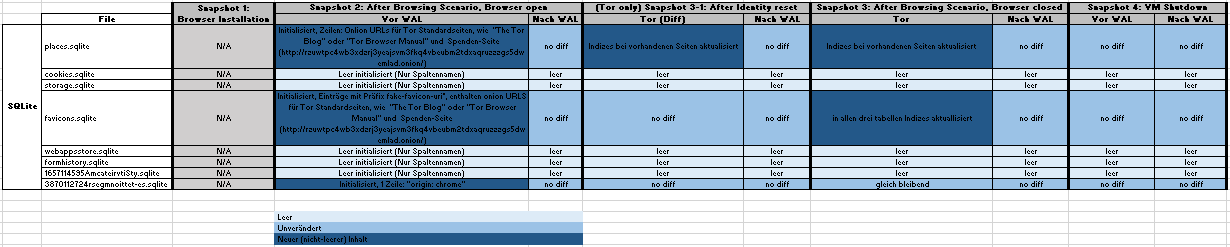
\includegraphics{bilder/tor-sqlite-table.png}}}
%	\label{chart:final-criteria}  
%	\caption{Comparison of found PB artifacts between RAM Dumps}
%\end{figure}
Nach Browser-Installation wurde noch keine SQLite-Datei angelegt (Snapshot 1).

Während des Browsing Szenarios wurden alle Datenbänkte initialisiert.
In places.sqlite wurden automatisch .onion URLs geschrieben, die zu Tor Standardseiten führen. Beispielsweise Seiten wie ``The Tor Blog`` oder ``Tor Browser Manual``.
Die gleichen Einträge wurden in der favicons.sqlite Datenbank geschrieben, mit dem Präfix ``Fake-favicon-uri``. Ein tatsächliches Icon wurde nicht in die Datenbank geschrieben. 
Weiterhin erhielt die ``remote settings`` Datenbank den gleichen Eintrag wie es bereits bei Firefox der Fall war. Der Eintrag enthält keine PB Artefakte.
Die restliche SQLite-Dateien wurden ohne Inhalt angelegt, nur die Spaltennamen wurden definiert.
Nach Durchführung der WAL Checkpoints bleiben Dateien unverändert.

Nachdem dem Tor-Browser eine ``Neue Identität`` zugewiesen wurde (Snapshot 3-1), wurden in places.sqlite die Indizes bei den eingetragenen Seiten aktualisiert. Die restlichen Dateien blieben unverändert. Das Schreiben der WAL-Dateien in die Hauptdatenbanken veränderte den Inhalt nicht.

Nach Schließen des Browsers (Snapshot 3-2) wurden in places.sqlite sowie favicons.sqlite erneut Indizes bei eingetragenen Seiten aktualisiert. Die restliche Dateien blieben unverändert, ebenso ergaben die WAL Checkpoints keine Veränderungen.

Nach Herunterfahren der VM (Snapshot 4) blieben alle Datenbanken unverändert. Auch nach Durchführung der WAL Checkpoints gab es keine neuen Inhalte.

Im Balkendiagramm \ref{chart:firefox-writefile-logfile1v21vs22} ist zu erkennen, dass die meisten Schreiboperationen im ersten Logfile stattfinden. Dort werden Dateien jeder Kategorie beschrieben. Das Schließen des Tor-Browsers führt zu mehr oder genauso vielen Schreiboperationen wie das Zuweisen einer ``Neuen Identität``. Keine der geschriebenen Dateien enthielt private Browsing Artefakte.
%*** TODO: Was noch? ***
\begin{figure}[h!]
	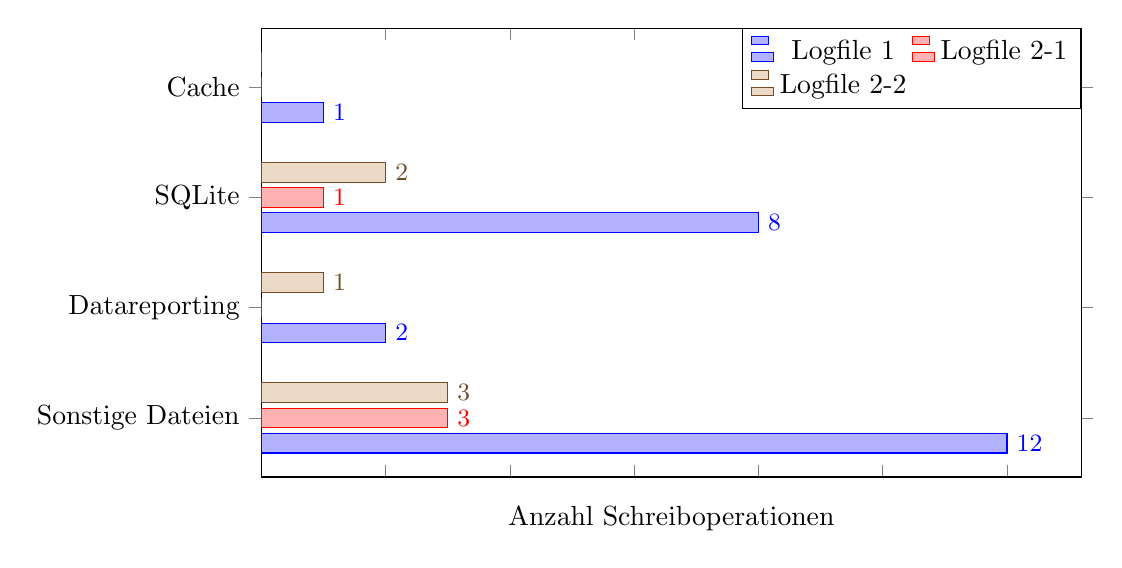
\begin{tikzpicture}
	\begin{axis}[
	xbar, 
	xmin=0,
	width=12cm, 
	height=12cm, 
	xlabel={Anzahl Schreiboperationen},
	y=1.4cm,
	symbolic y coords={Sonstige Dateien,Datareporting,SQLite,Cache},
	ytick=data,
	xticklabels={,,},
	nodes near coords style={font=\small},
	nodes near coords={\pgfmathfloatifflags{\pgfplotspointmeta}{0}{}{\pgfmathprintnumber{\pgfplotspointmeta}}},
	bar width=.25cm,
	enlarge y limits={abs=3*\pgfplotbarwidth},
	legend style={
		at={(1,1)},
		anchor=north east
	},
	legend columns=2,
	scaled x ticks=false
	]
	\addplot coordinates {(12,Sonstige Dateien) (2,Datareporting) (8,SQLite) (1,Cache)};
	\addplot coordinates {(3,Sonstige Dateien) (0,Datareporting) (1,SQLite) (0,Cache)};
	\addplot coordinates {(3,Sonstige Dateien) (1,Datareporting) (2,SQLite) (0,Cache)};	
	\legend{Logfile 1, Logfile 2-1, Logfile 2-2}
	\end{axis}
	\end{tikzpicture}
	\caption{Tor Anzahl Schreiboperationen Logfile 1 vs Logfile 2-1 vs Logfile 2-2, geordnet nach Kategorie}
	\label{chart:firefox-writefile-logfile1v21vs22}
\end{figure}
%\begin{figure}[h!]
%	\centerline{\resizebox{\linewidth}{!}{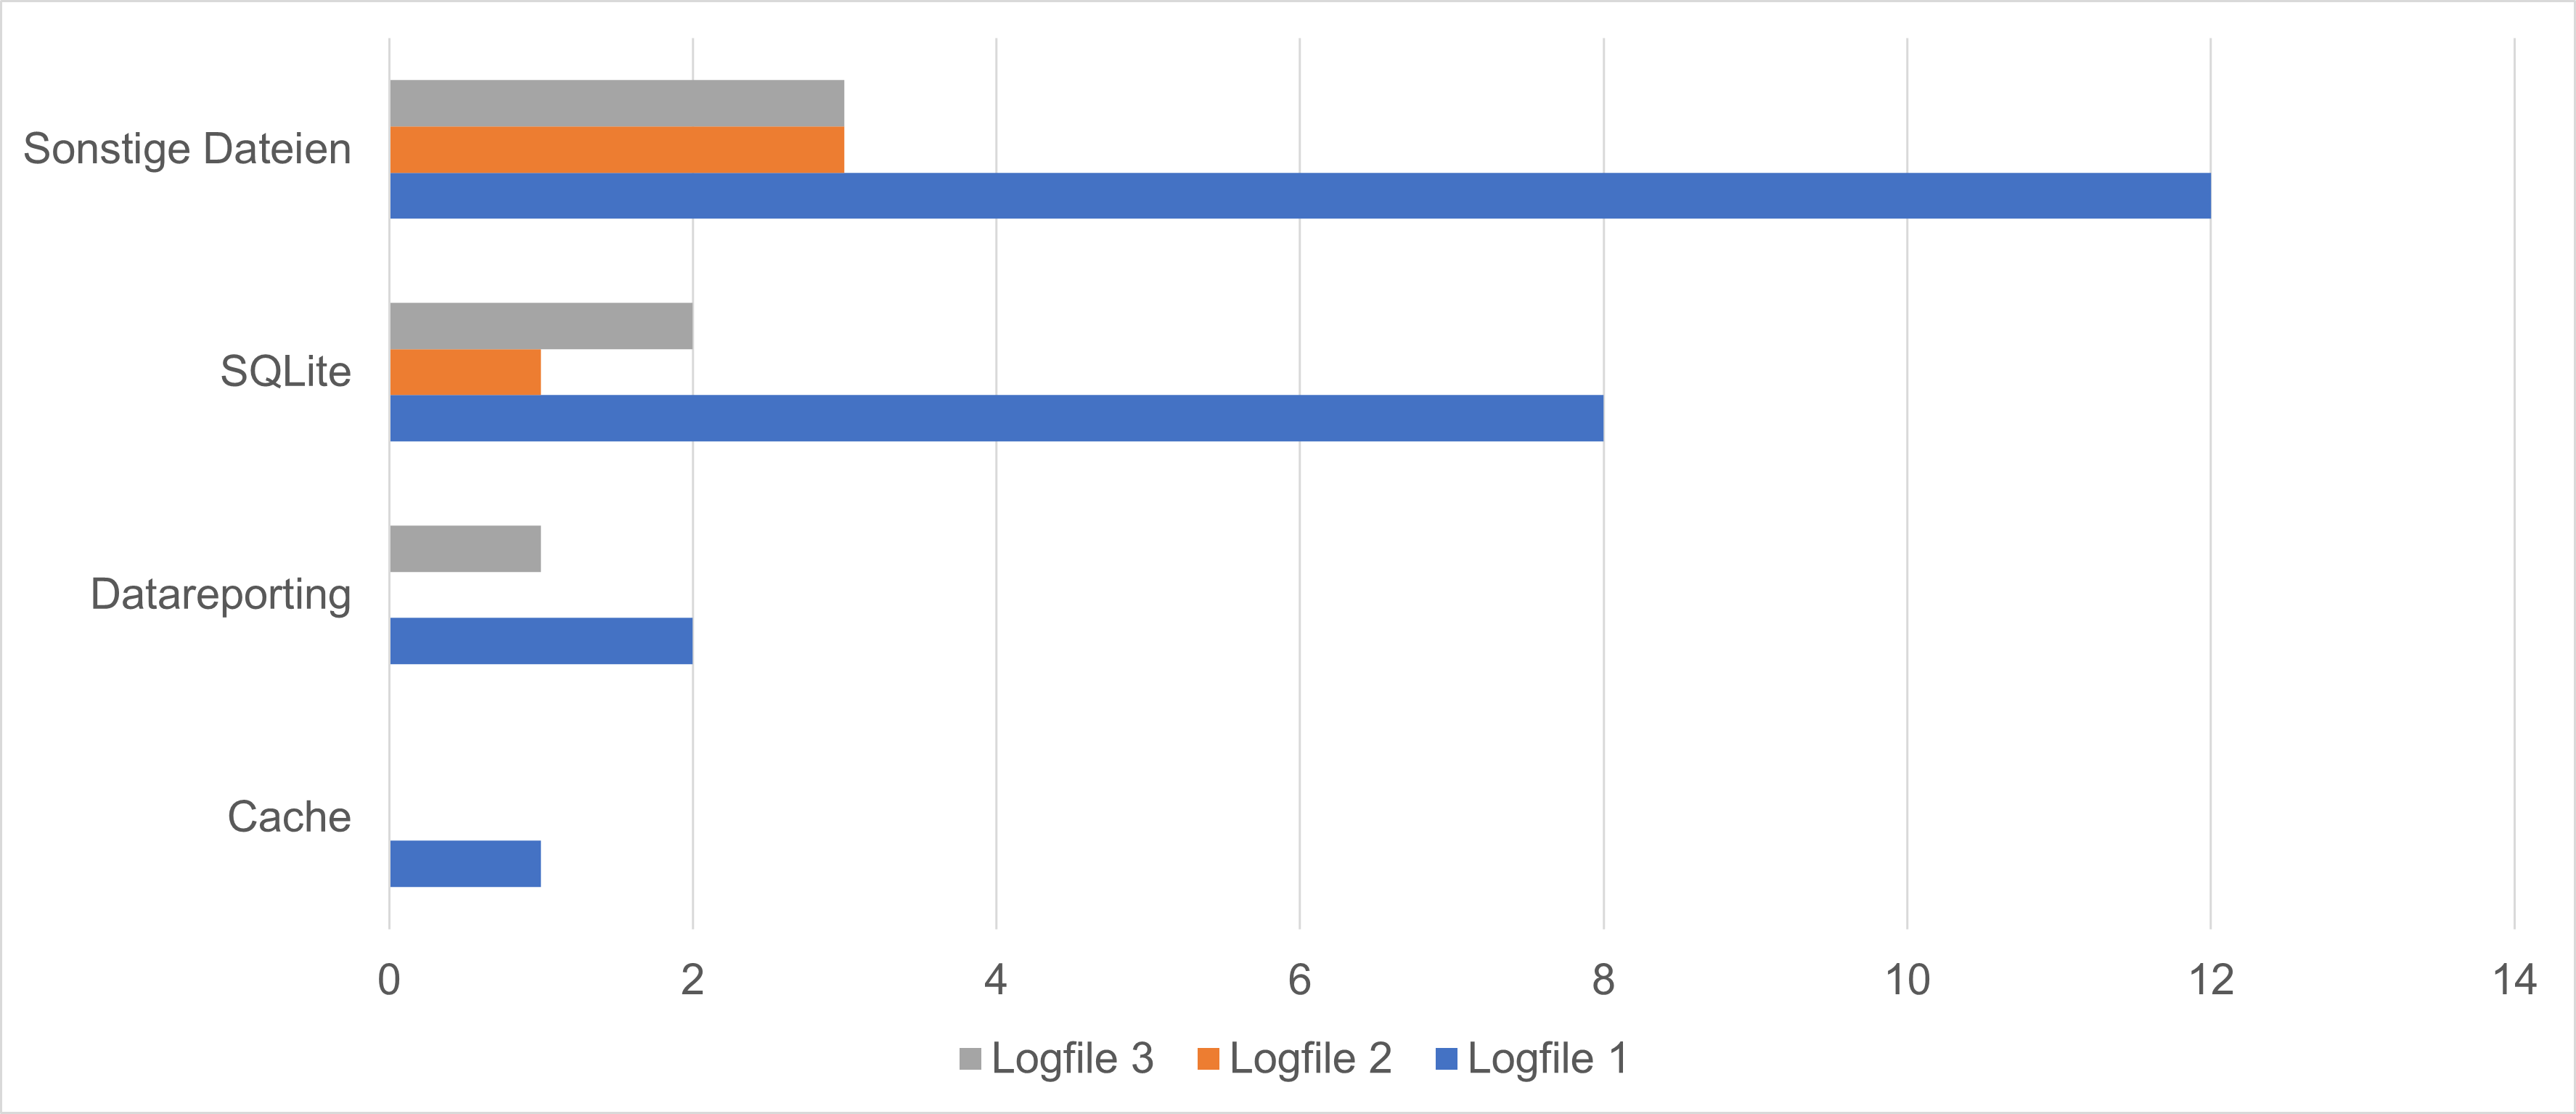
\includegraphics{bilder/tor-bar-chart-logfile1vs2cs3.png}}}
%	\label{chart:final-criteria}  
%	\caption{Comparison of found PB artifacts between RAM Dumps}
%\end{figure}

%Literatur:
%	o no traces were found in “common locations” \cite{Montasari.2015}
%		>  “places.sqlite”, “webappsstore. sqlite”, “sessionstore.bak”, “search.json” and “nssckbi.dll”
%	o	Safebrowsing: Alle Dateien in /safebrowsing-updating/ nicht relevant. Dort nur .vlpset und .sbstore Dateien. Speichern 256-Bit Hash von URLs, die auf SafeSearch Blacklist stehen 
%	o	Cache-Dateien: drei Caches: startupCache, jumpListCache (beide enthalten Binärdateien ohne Browsing Artefakte) und cache2 (können mit MozillaCacheView untersucht werden, enthalten keine Browsing Artefakte)
%	o	SQLite Datenbanken: Sqlite Dateien erst ohne WAL Dateien untersuchen, Danach mit sqlite3 Konsole: WAL in Datenbank schreiben mit: PRAGMA wal\_checkpoint; places.sqlite besonders relevant, da dort Browser in public Modus Browsing URLs verwaltet (Am besten hier vergleich mit Public Browsing machen)	
%		> \cite{Fayyad.2021} for Mozilla Firefox, 7 database files were recovered: cookies.sqlite-shm, places.sqlite-shm, prefs.js etc.
%		> \cite{Muir.2019} The two SQLite databases used by Firefox to track cookies and history (cookies.sqlite und places.sqlite) were both recoverable from the file system after deletion	
%		Ergebnisse stehen im Gegensatz zu \cite{Hedberg.2013} :
%			o	Chrome und Firefox: Einträge in places.sqlite + history.sqlite DB gefunden während PB! (Noch aktuell??)
%		Sonderfall: SQlite DB-Crash \cite{Hedberg.2013}
%			> WAL Files/Journal Files bei Crash gefunden -> Kann genutzt werden um zu beweisen, dass privater Browser genutzt wurde
%			> Daher: WAL Rollback mit sqlite3	
%	o	Jsonlz4 \& balkz4: Enthalten komprimierte Firefox-Sessions, jsonlz4 Dateien können mit Tool ``entkomprimiert`` werden: https://www.jeffersonscher.com/ffu/scrounger.html


\subsection{Uncommon Locations}
\label{subsection:appendix-tor-uncommon-locations}

\subsubsection*{Analyse mit Autopsy - Kategorisierte Dateien}
\label{subsubsection:appendix-tor-uncommon-locations-autopsy}

Wie bei Firefox in Kapitel \ref{subsubsection:appendix-firefox-uncommon-locations-autopsy} wurde keine der kategorisierten Dateien gelöscht. Somit befanden sich im letzten Festplatten-Image des Snapshots 4 alle kategorisierten Dateien der vorherigen Festplatten-Images

\paragraph*{Web Bookmarks}
Wie in Abbildung \ref{img:tor-web-bookmarks} gezeigt, wurden nur in der Datei \texttt{Bing.url} ein Leesezeichen zur Bing-Startseite gefunden. Diese Datei wurde im Festplatten-Image des ersten Snapshots geschrieben.
\begin{figure}[h!]
	\centerline{\resizebox{\linewidth}{!}{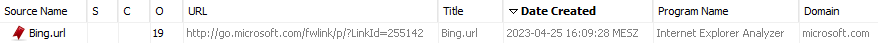
\includegraphics{bilder/cfv_tor_autopsy_web_bookmarks.png}}} 
	\caption{Tor: Von Autopsy als ``Web Bookmarks`` kategorisierte Dateien}
	\label{img:tor-web-bookmarks} 
\end{figure}

\paragraph*{Web Cookies}
Im Festplatte-Image des ersten VM-Snapshots wurden die in Abbildung \ref{img:tor-web-cookies} gezeigten neun Cookies-Einträge in die Datenbank des vorinstallierten Edge Browsers geschrieben. Dabei handelt es sich um Cookies für die Bing- und Outlook-Startseite.
\begin{figure}[h!]
	\centerline{\resizebox{\linewidth}{!}{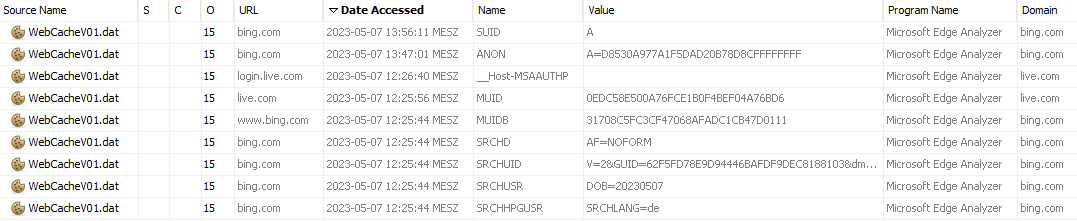
\includegraphics{bilder/cfv_tor_autopsy_web_cookies.png}}} 
	\caption{Tor: Von Autopsy als ``Web Cookies`` kategorisierte Dateien}
	\label{img:tor-web-cookies} 
\end{figure}

\paragraph*{Web History}
Zwei Einträge mit Browsingverläufen wurden im Festplatten-Image des ersten VM-Snapshots in der Datei \texttt{WebCacheV01.dat} geschrieben. Wie in Abbildung \ref{img:tor-web-history} gezeigt, handelt es sich dabei zweimal um die Outlook-Startseite, obwohl diese nie bei der Versuchsdurchführung geöffnet wurde. Wie bei Firefox wurden in der Datei ebenfalls die zum Analyserechner über den gemeinsamen Ordner transportierten Process Monitor Logfiles gespeichert.
\begin{figure}[h!]
	\centerline{\resizebox{\linewidth}{!}{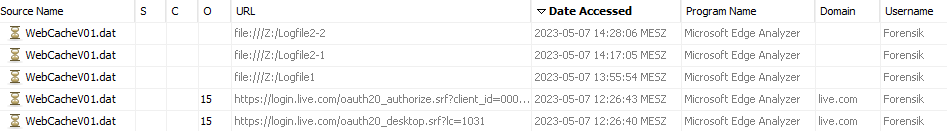
\includegraphics{bilder/cfv_tor_autopsy_web_history.png}}}
	\caption{Tor: Von Autopsy als ``Web History`` kategorisierte Dateien}
	\label{img:tor-web-history}  
\end{figure}

\paragraph*{Web Categories}
Autopsy klassifizierte im Festplatten-Image des ersten VM-Snapshots den Eintrag \texttt{bing.com} als ``Suchmaschine``  und \texttt{live.com} als ``Web-Email``, gezeigt in Abbildung \ref{img:tor-web-categories}.
Es gab keine zusätzlichen Einträge in dieser Kategorie in den Festplatten-Images der restlichen Snapshots.
\begin{figure}[h!]
	\centerline{\resizebox{\linewidth}{!}{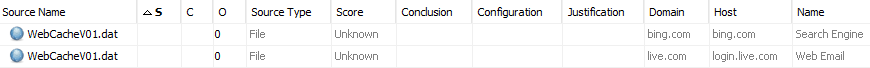
\includegraphics{bilder/cfv_tor_autopsy_web_categories.png}}} 
	\caption{Tor: Von Autopsy als ``Web Categories`` kategorisierte Dateien}
	\label{img:tor-web-categories} 
\end{figure}
		
Somit wurden in den von Autopsy kategorisierten Dateien keine PB Artefakte entdeckt. Weiterhin gab es verglichen mit der Analyse der Common Locations keine neuen Erkenntnisse. Autopsy erkannte nicht die in der places.sqlite Datenbank geschriebenen .onion-URLs der Tor-Standardseiten.

%Literatur:
%	o	Autopsy Keywortsuche: 
%		>	In alles Snapshots ergebnislos (keine Keyword-Hits
%		-->	In Literatur: Autoren fanden Ergebnisse in pagefile.sys 
%			> Autopsy: websites and some of the keywords found in hidden file called “pagefile.sys” \cite{Mahlous.2020}
%			o \cite{Montasari.2015} traces were found in: 
%				> However, on investigating the “pagefile.sys”, some entries were discovered
%				> Using the “data carving” technique, profile picture was recovered
%			o \cite{Said.2011} 
%				> Examining pagefile.sys showed some positive hits 			
%		--> Evtl. hier zeigen, was gefunden werden kann, wenn RAM reduziert
%		--> Aber auf Problem hinweisen, dass gefundener String in pagefile nicht direkt Browser zugeordnet werden kann
%		> \cite{Gabet.2018}	Firefox only produced three recoverable artefacts as reported by both tools (FTK, Autopsy) --> Artefakte werden nicht genannt!
%		> \cite{Muir.2019} Autopsy Keyword Suche nach Suchbegriffen: unallocated space
%		> Autopsy Carving Module (\$Carved): \cite{Muir.2019}
%			•	When searching for the string ’clot’ from the browsing protocol, six .dll, .edb and .reg files were discovered in unallocated space.
%			•	Further searching of unallocated space uncovered references to the Tor installation directory and the obfs4 bridging IP addresses
%			•	browsing data found in NTUSER.DAT was also replicated in unallocated space.
%	o	Autopsy PlugIns:
%		>	*** TODO: Hier Liste mit PlugIns ***

\subsection{Registry}

\subsubsection*{Process Monitor SetValue Operations}

Bei Betrachtung als Common Locations werden gemäß Methodik in Kapitel \ref{subsection:methodik-datenanalyse-registry} alle ``SetValue`` Schreiboperationen in den Process Monitor Logfiles für die Prozesse ``tor.exe`` und ``firefox.exe`` untersucht. 

Dabei wurden die gleichen beiden Registry Keys identifiziert, wie bei der Untersuchung der Firefox Registry in Kapitel \ref{subsubsection:appendix-firefox-registry-processmonitorsetvalue}: \texttt{PreXULSkeletonUISettings} und \texttt{Business Activity Monitoring}. In keinem Registry-Key befinden sich PB Artefakte.
Wie in Abbildung \ref{chart:tor-registy-css-vs-bam} dargestellt, wurden beide Registry Keys annähernd gleich oft geschrieben. Bei Vergleich der drei Process Monitor Logfiles 1, 2 und 3 nimmt Anzahl der Registry ``SetValue``-Operationen bei Logfile 2 und 3 kontinuierlich ab.

\begin{figure}[h!]
	\resizebox{\linewidth}{!}{
	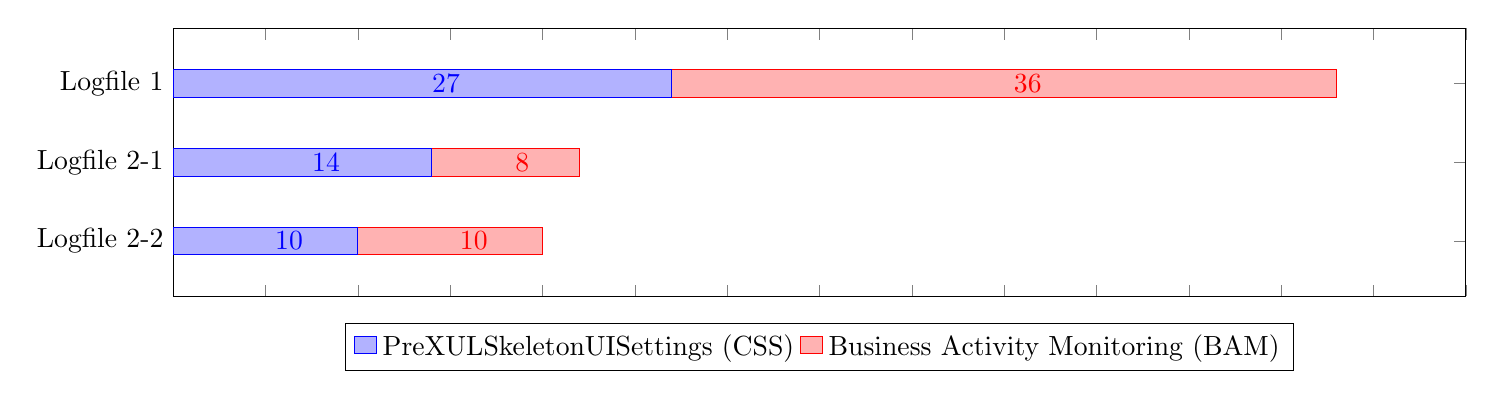
\begin{tikzpicture}
		\begin{axis}[
		xbar stacked,
		width=18cm, 
		height=12cm, 
%		ylabel style={align=center}, ylabel=RAM-Dump 1,
		y=1cm,
		enlarge y limits={abs=2*\pgfplotbarwidth},
		symbolic y coords={Logfile 2-2,Logfile 2-1,Logfile 1},
		ytick=data,
		xticklabels={,,},
        xmin = 0,
        xmax = 70,
		nodes near coords, 
		nodes near coords align={horizontal},
		legend style={
			at={(0.5,-0.1)},
			anchor=north
		},
		legend columns=2,
		scaled x ticks=false
		]
			\addplot coordinates {
			(10,Logfile 2-2) (14,Logfile 2-1) (27,Logfile 1)
			};
			\addplot coordinates {
			 (10,Logfile 2-2) (8,Logfile 2-1) (36,Logfile 1)
			};
			\legend{PreXULSkeletonUISettings (CSS), Business Activity Monitoring (BAM)}
		\end{axis}
	\end{tikzpicture}
	}	
	\caption{Tor Registry ``SetValue`` Operationen in den Process Monitor Logfiles 1, 2-1 und 2-2}
	\label{chart:tor-registy-css-vs-bam}
\end{figure}

%\begin{figure}[h!]
%	\centerline{\resizebox{\linewidth}{!}{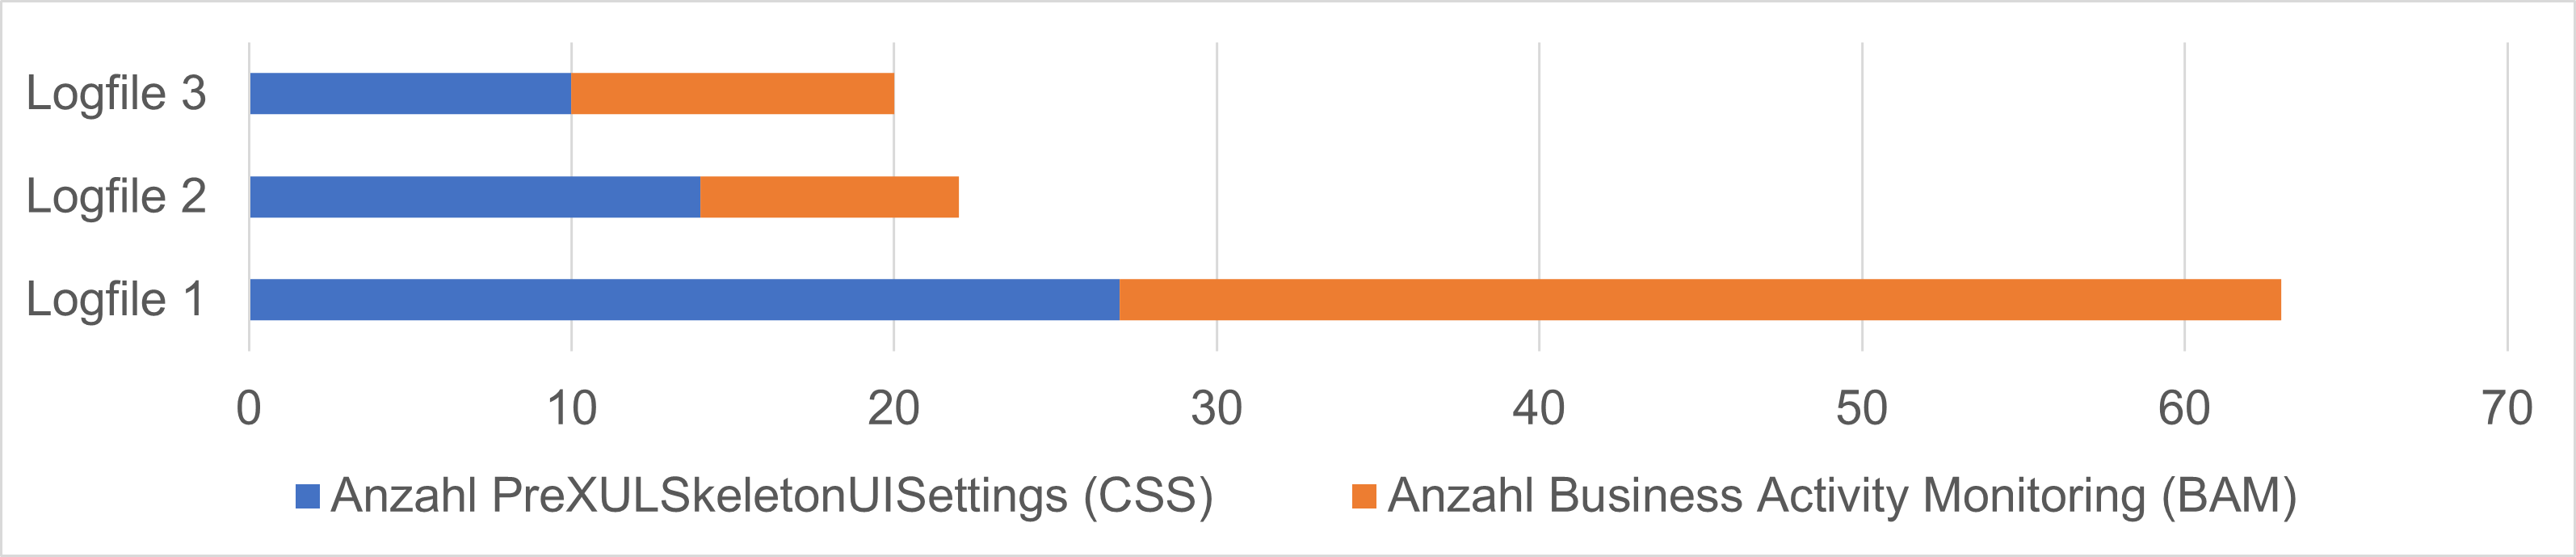
\includegraphics{bilder/tor-registry-stacked-bar-chart.png}}}
%	\label{chart:final-criteria}  
%	\caption{Comparison of found PB artifacts between RAM Dumps}
%\end{figure}

\subsubsection*{Stringsuche in Registry Hives}
Bei Betrachtung der Registry als Uncommon Locations, wurden die in Tabelle \ref{tab:windows-registry-hives} im Kapitel \ref{subsection:methodik-datenanalyse-registry} aufgelisteten Registry-Hives mithilfe des Registry Explorers untersucht. 
Weder in den System-Hives noch in den User-Hives konnte in keinem Festplatten-Image PB Artefakte identifiziert werden. 

%Literatur:
%	>	Auf Autor verweisen: angeblich in Shellactivities Ergebnisse. --> Nicht mehr vorhanden in aktueller Version (Verweis auf E-Mail)
%	>	Process Monitor/Regshot zeigen keine relevanten Key-Änderungen
%	> \cite{Muir.2019}: Autopsy Keyword Suche nach Suchbegriffen: Ergebnisse in \%SystemRoot\%Minidump NTUSER.DAT, ntuser.dat.LOG1 (a log of changes to NTUSER.DAT)
%	> Zentral: shellactivites Key:	NTUSER.DAT --> “shellactivities” key \cite{Muir.2019}
%	> \cite{Rochmadi.2017} Detection of registry changes helps to determine what the appropriate plugin is used to search for digital evidence using volatility memory forensic:
%	- RegQueryValue:	HKCU/Software/Microsoft/Windows/CurrentVersion/InternetSettings/Connections/DefaultConnectionSettings
%	- RegCloseValue: 	HKCU/Software/Microsoft/Windows/CurrentVersion/InternetSettings/Connections
%	- IRP\_MJ\_READ: C:/pagefile.sys

	
%		\addtocontents{toc}{\endgroup}
\end{appendices}